%%%%%%%%%%%%%%%%%%%%%%% file template.tex %%%%%%%%%%%%%%%%%%%%%%%%%
%
% This is a template file for The European Physical Journal
%
% Copy it to a new file with a new name and use it as the basis
% for your article
%
%%%%%%%%%%%%%%%%%%%%%%%% Springer-Verlag %%%%%%%%%%%%%%%%%%%%%%%%%%
%
\begin{filecontents}{leer.eps}
%!PS-Adobe-2.0 EPSF-2.0
%%CreationDate: Mon Jul 13 16:51:17 1992
%%DocumentFonts: (atend)
%%Pages: 0 1
%%BoundingBox: 72 31 601 342
%%EndComments
gsave
72 31 moveto
72 342 lineto
601 342 lineto
601 31 lineto
72 31 lineto
showpage
grestore
%%Trailer
%%DocumentFonts: Helvetica
\end{filecontents}
%
\documentclass[epj]{svjour}
% Remove option referee for final version
%
% Remove any % below to load the required packages
%\usepackage{latexsym}
\usepackage{amsmath,amssymb,amsfonts} % AMS math & symbols
\usepackage{bm}              % bold math
\usepackage{amscd}           % for extensible arrows (e.g., limits)
\usepackage{graphics}
\usepackage{hhline,multirow} % for nicer tables
\usepackage{dcolumn}         % Align table columns on decimal point
\usepackage{color}
% etc
%%%%%%  Definitions   %%%%%%%%%%%

\newcommand{\eqeqref}[1]{Eq.~\eqref{#1}}
\newcommand{\eqseqref}[1]{Eqs.~\eqref{#1}}
\newcommand{\refref}[1]{Ref.~\cite{#1}}
\newcommand{\refsref}[1]{Refs.~\cite{#1}}
\newcommand{\secref}[1]{Sec.~\ref{#1}}
\newcommand{\appref}[1]{App.~\ref{#1}}
\newcommand{\figref}[1]{Fig.~\ref{#1}}
\newcommand{\tabref}[1]{Table~\ref{#1}}

\newcommand{\beq}{\begin{equation}}
\newcommand{\eeq}{\end{equation}}
\newcommand{\bea}{\begin{eqnarray}}
\newcommand{\beas}{\begin{eqnarray*}}
\newcommand{\beau}[1]{\begin{equation} \label{#1} \begin{array}{rcl}}
\newcommand{\eea}{\end{eqnarray}}
\newcommand{\eeas}{\end{eqnarray*}}
\newcommand{\eeau}{\end{array} \end{equation}}
\newcommand{\bay}{\begin{array}}
\newcommand{\eay}{\end{array}}
\newcommand{\bals}{\begin{align*}}
\newcommand{\eals}{\end{align*}}

\newcommand{\ds}{\displaystyle}
\newcommand{\emnr}{\epsilon_{\mu\nu\rho}}
\newcommand{\erre}{{\hbox{{\rm I}\hspace{-.2em}\hbox{\rm R}}}}
\newcommand{\bbeta}{\mbox{\boldmath$\beta$\unboldmath}}
\newcommand{\bb}{{\bf b}}

\newcommand{\cL}{{\mathcal L}}
\newcommand{\lora}{{\longrightarrow}}
\newcommand{\Lora}{{\Longrightarrow}}
\newcommand{\Lolra}{{\Longleftrightarrow}}
\newcommand{\Lra}{{\Leftrightarrow}}
\newcommand{\Ra}{{\Rightarrow}}
\newcommand{\ra}{{\rightarrow}}
\newcommand{\lra}{{\leftrightarrow}}

\newcommand{\bra}[1]{\langle #1 \vert}
\newcommand{\ket}[1]{\vert #1 \rangle}
\newcommand{\scal}[2]{\langle #1 \vert #2 \rangle}
\newcommand{\matel}[3]{\langle #1 \vert #2 \vert #3 \rangle}
\newcommand{\vev}[1]{\langle #1 \rangle}
\newcommand{\vav}[1]{\matel{0}{#1}{0}}
\newcommand{\interno}[2]{\left( #1 , #2 \right)}
\newcommand{\com}[2]{\left[ #1, #2 \right]}

\newcommand{\intmom}[1]{\int {{d^3 #1} \over {(2 \pi)^3}} \,}
\newcommand{\esp}[1]{\, e^{\,\,\textstyle {#1}}}
%\newcommand{\esp}[1]{\, \mbox{\large \sl e}^{\textstyle \, #1}}
\newcommand{\In}[2]{ \left. #1 \right| _{#2} }
\newcommand{\Inp}[1]{ {}_{\displaystyle | \scriptstyle #1 } }

\newcommand{\nbar}{{\overline n}}
\newcommand{\mbar}{{\overline m}}
\newcommand{\xbar}{{\overline x}}

\newcommand{\DD}{{\mathcal D}}
\newcommand{\EE}{{\mathcal E}}
\newcommand{\OO}{{\mathcal O}}
\newcommand{\PP}{{\mathcal P}}
\newcommand{\RR}{{\mathcal R}}

\newcommand{\qhat}{{\hat q}}

%\usepackage{setspace}
%\doublespacing
%
\begin{document}
%
\title{A Monte Carlo Simulation of Parton Quenching \\ in Cold Nuclear Matter}
\author{Rapha\"el Dupr\'e \inst{1,}\thanks{dupre@ipno.in2p3.fr} 
\and Alberto Accardi \inst{2,3,}\thanks{accardi@jlab.org}}

%
\institute{
Institut de Physique Nucl\'eaire Orsay, CNRS-IN2P3, Universit\'e Paris-Sud, 
France \and Hampton University, Hampton, VA 23668, USA \and
Thomas Jefferson National Accelerator Facility, Newport News, VA 23606, USA}
%
\date{Received: date / Revised version: date}
% The correct dates will be entered by Springer
%
\abstract{
We present a Monte-Carlo simulation of hadron quenching in semi-inclusive electron-nucleus collisions, and compare its results with experimental data on hadron multiplicity ratios and transverse momentum broadening from the HERMES experiment. The simulation is based on the Pythia event generator, to which we add nuclear effects, such as the Fermi motion of nucleons, the parton energy loss and the parton transverse momentum broadening. Fermi motion effect appear in our simulation to be non negligible for experiments performed at Jefferson Lab energies and also relevant, for selected observables, for the HERMES experiment.
The energy loss of final state partons propagating through the nuclear medium is implemented following the quenching weight formalism by Salgado and Wiedemann. Different ways of treating the transverse parton momentum broadening are discussed. 
%We obtain our best result for the combined description of both multiplicity ratios and transverse momentum broadening from HERMES by using a Monte-Carlo method completely based on the Salgado and Wiedemann calculation. 
Hadron multiplicities and transverse momentum broadening are typically well described by using a transport coefficient $\qhat = 0.36\ \text{GeV}^2/ \text{fm}$. One exception is the dependence of the hadron multiplicity on the virtual photon energy, $\nu$, which is possibly uncovering the limitations in the adopted theoretical description of the parton energy loss process.
} %end of abstract
%
\maketitle
%
\section{Introduction}
\label{intro}

Parton energy loss in the nuclear medium has been extensively used in the last decade as a sensitive probe of the Quark-Gluon Plasma (QGP) created in heavy ion collisions at the Relativistic Heavy Ion Collider (RHIC) \cite{Adams:2005dq,Adcox:2004mh} and the Large Hadron Collider (LHC) \cite{Aamodt:2010jd,CMS:2012aa}. The idea is that a hard scattered parton traverses the produced QGP and interacts with its color field. The subsequent in-medium parton rescattering causes parton momentum broadening and energy loss by non-Abelian gluon radiation. In turn, this manifest itself in a suppression of high-energy hadron and jet production, and in a broadening of the hadron momentum spectrum or a modification of the jet shape. These effects are often collectively referred to as ``jet quenching''.
The properties of the medium can then be reconstructed from the nuclear modification of hadron and jet production once the in-medium parton propagation dynamics is theoretically under control. 

Most of the theoretical and phenomenological work in recent years has been devoted to the study of parton energy loss in ``hot QCD matter'' with the goal of utilizing hadron quenching and momentum broadening as a tomographical probe of the QGP \cite{Majumder:2010qh}. However, considerable theoretical uncertainties exist within and among the various energy loss calculations, and these need to be clarified to turn jet quenching into a truly quantitative tool for QGP characterization \cite{Armesto:2011ht}. In this perspective, studying parton propagation in ``cold nuclear matter'' \cite{Accardi:2009qv} provides one with the possibility to test theoretical calculations and assumptions in a known medium -- a nucleus target of known density and composition. Examples are nuclear modification of hadron and jet production in $e+A$ collisions, as well as of lepton pair production in $p+A$ collisions. In either case, and contrary to $A+A$ collisions, the exchanged hard four momentum is well constrained experimentally and the multiplicity in the final state is small providing an ideal theoretical and experimental environment. Thus the approximation schemes and calculation techniques adopted in the different energy loss models (some of which are in fact derived for $e+A$ collisions and applied under simplifying assumptions to propagation through hot QCD matter) can be tested on actual experimental data, providing a set of benchmarks that go beyond those afforded by the use of a theoretical ``brick'' of QCD matter \cite{Armesto:2011ht}. 

Hadron quenching in $e+A$ collisions is important not only as a test of energy loss models, but also to study the color field of a nucleus. Indeed, the transverse momentum broadening due to the energy loss can be linked 
to the gluon distribution~\cite{Baier:1996sk} and, eventually, to the gluon 
saturation scale~\cite{Kopeliovich:2010aa}. More in general, parton propagation
can be described in terms of a number of ``transport coefficients'' characterizing the medium and controlling the parton's transverse momentum broadening, longitudinal drag, and diffusion \cite{Majumder:2008zg,Majumder:2007hx,Idilbi:2008vm,other-transport-coefficients?}. These can be given a field theoretical definition in terms of gauge invariant gluon and quark nuclear correlators, that provide a first-principles characterization of the medium the parton is propagating through and can be  extracted from experimental data on nuclear modifications of hadron and jet production. The possibility to calculate transport coefficients in lattice QCD has been recently discussed \cite{Majumder:2012sh}. Finally, it was recently shown that the transverse momentum dependence of azimuthal asymmetries in $e+A$ collisions is sensitive to the relative shape of various transverse momentum dependent parton distributions functions of the nucleons \cite{Gao:2010mj,Song:2010pf,Song:2013sja}. So to speak, one can use the nucleus as a microscope to study the structure of its nucleons.


In order to study parton (rather than hadron) propagation in cold nuclei, one needs to select events with large longitudinal momentum of the exchanged virtual photon compared to the nucleus, to ensure that the propagating quark has a large energy and the hadronization process is boosted outside the nucleus. In $e+A$ collisions this requires a large enough center of mass energy range  (data are available from JLab at 5 GeV, HERMES at 27 GeV and EMC at 100-280 GeV electron beam energy, and in the future at even higher energy from the planned Electron Ion Collider \cite{Accardi:2009qv}). In Drell-Yan measurements the hadronization problem is absent and one can isolate parton energy loss from it. However the cross section is also affected by initial state effects such as quark antishadowing that can obscure energy loss effects. Therefore in this article we will restrict our analysis to $e+A$ collisions.

The amount of information that can be obtained from experimental data on nDIS is, however, directly limited by our capability to infer the parton energy loss and transverse momentum broadening from the observed hadronic spectra. The available analytic calculations \cite{Accardi:2009qv} are limited in this respect by the underlying collinear factorization approximation, in which 
the hadron moves in the same direction as the parton it originates from, and carries a fraction of its momentum determined by its fragmentation function. In reality the hadronization process is more complex, and it is important to account in a more realistic way for fragmentation effects on an event by event basis, both for a more accurate mapping of hadron to parton energy loss effects and for a more precise implementation of the experimental cuts.


In this perspective, we have developed a Monte Carlo simulation of hadron quenching for nuclear Deep Inelastic Scattering (nDIS). While for the case of hot QCD matter there exist a large number of sophisticated simulations \cite{some-review-with-hot-MCs,Buzzatti:2010ck}, none has so far been developed for $e+A$ collision, with the exception of that in Ref~\cite{Majumder:2009zu} that however does not include hadronization of the hard-scattered partons. The simulation we describe in this article is based on the Pythia event generator, which takes care of the hard photon-parton interaction at the nucleon level, and uses the Lund string model for parton-to-hadron fragmentation with full account of energy-momentum conservation. Final state nuclear effects are then treated in a pure parton energy loss framework, with neglect of hadron absorption effects. As discussed this can be easily motivated at high enough hadron energy, since hadron production is boosted outside of the nuclear medium (although just how high this energy should be has not yet been experimentally determined \cite{Accardi:2011mz}). As for initial state nuclear effects, we include Fermi motion and binding energy corrections {\bf (do we?) -- [AA] this has to be checked in the code: if a delta-function imposing that the (A-1) spectaor is on-shell is included in the kinematics then yes, we are including binding although in an approximate way.  }, but neglect nuclear modifications of parton distributions because these largely cancel between the numerator and denominator of the chosen observables. In this first effort we focus on methodology and test our simulation on a limited set of HERMES data. A detailed phenomenological analysis of all available experimental data is left for future work.


The paper is structured as follows.....................



\section{Observables and kinematic variables of interest}


\begin{table*}[tbp]
  \center
  \begin{tabular}{rclcll} 
    \hline 
    \it Variable & & \multicolumn{2}{l}{\it Invariant} & {\it
      Target rest frame} & \\\hline
    $Q^2$ & = & $-q^2$ & & 
      & \parbox[t]{4.9cm}{\raggedright Negative four-momentum 
      squared of the virtual photon.}\\
    $\nu$ & = & $\frac{q\cdot P}{\sqrt{P^2}}$ & = & $E-E'$ 
      & \parbox[t]{4.9cm}{\raggedright Energy of the virtual  
      photon in the target rest frame.}\\
    $x$ & = & $\frac{-q^2}{2P\cdot q}$ & &
      & \parbox[t]{4.9cm}{\raggedright Bjorken scaling variable.\\ \ }\\
    $W^2$ & = & $(P+q)^2$ \quad & = & $M^2 + 2M\nu - Q^2$ \qquad
      & \parbox[t]{4.9cm}{\raggedright  Invariant mass squared of 
      the total hadronic final state.
      \vskip.2cm}\\
    $z_h$   & = & $\frac{p\cdot P}{q\cdot P}$ & = & $\frac{E_h}{\nu}$ 
      & \parbox[t]{4.9cm}{\raggedright Fraction of the virtual photon 
      energy carried by the  hadron.}\\ \hline
  \end{tabular}\\
  \caption{Definitions of the kinematic variables for semi-inclusive
    DIS. The Lorentz invariant definition and its form in the target
    rest frame are provided. Note that $x= Q^2 / (2M\nu)$
    independently of the chosen reference frame.
{\bf [AA] Use rather the simplified Table from Accardi et al. review}
 } 
  \label{tab:DISkinvar}
\end{table*}


\begin{figure}[tbp]
  \centering
  \resizebox{0.4\textwidth}{!}{
    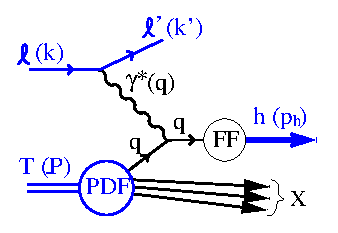
\includegraphics{fig/DIS-kinematics.eps} }
  \caption{Semi-inclusive hadron production in deep inelastic scattering on a 
target $T$ in the pQCD factorization approach at leading order. Parton 
distribution functions (PDF) and fragmentation functions (FF) represent the 
non-perturbative input simulated using Pythia.
{\bf [AA] we need a figure without the parton scattering level, and that does not use Fragmentation Functions. Essentially the same, but with the photon scattering on the proton ``blob'', with a hadron $h$ and rest $X$ coming out straight from it.}
}
  \label{fig:DIS}
\end{figure}

The semi-inclusive DIS process is depicted in Fig.~\ref{fig:DIS} alongside the definition of the kinematic variables of interest.The variables $x,\nu$ and $Q^2$ are related by  $x = Q^2/(2M\nu)$, and in studies of medium modification of hadron production, it is customary to choose the 4-momentum exchange $Q^2$  and $\nu$ (rather than $x$) as independent variables. The reason is that the boost of the hadronization process from the hadron rest frame to the laboratory rest frame is controlled by the energy of the hard scattered parton, and this is proportional to $\nu$. The hadron transverse momentum is defined with respect to the virtual photon direction.

It is interesting to remark the differences relative to hadronic (in particular heavy ion) collisions. 
In DIS one can experimentally measure all the listed variables, especially $\nu$ and $z_h$. At leading order (LO) in perturbation theory. $\nu$ is equal to the energy of the scattered parton, and $z_h$ is equal to the fraction of (light-cone) momentum carried away by hadron into which the parton fragments. Thus one has an almost direct control on the parton level kinematics, that is not achievable in hadronic collisions because, contrary to the incident and scattered electron, initial and final state partons are not observables.
Thus, the initial conditions for the parton as it travels through the nuclear medium and loses its energy are under experimental control. Finally, in hadronic collisions, transverse momenta are measured relative to the beam axis, rather than the to the four momentum exchange, and it is important to not mistake this with the homonym variable in DIS; in particular, the hadron energy in nDIS is the analog of $p_T^h$ in mid-rapidity hadron production in hadronic collisions, and $p_T^h$ in DIS is analogous to the transverse momentum of a hadron with respect to the jet axis. 

The observables we are interested in are the multiplicity ratio and the 
transverse momentum broadening of the produced hadron. The hadron multiplicity ratio is defined as a double ratio
\begin{equation}
R^h_A = \frac{\left({N_h/N_e}\right)_A }{ \left({N_h/N_{e}}\right)_{D}},
\end{equation}
with $N_e$ the number of electron scattered from the target and $N_h$ the 
number of hadrons detected in coincidence with the scattered electron measured on a target of atomic number $A$ in the numerator and on a Deuteron in the denominator. In the absence of nuclear modification of hadron production, this ratio would be one and any deviation from that number indicates nuclear effects.
%
The second observable of interest is the hadron transverse momentum broadening. It is defined as the difference
\begin{equation}
\Delta \langle P_T^2 \rangle = \langle p_T^2 \rangle_A - \langle p_T^2 \rangle_{D},
\end{equation}
of the mean transverse momentum squared $\langle p_T^2 \rangle_A$ the mean $p_T^2$ of hadrons produced off a target $A$ and off the Deuteron. This quantity is typically positive, and indicates that the parton or the hadrons are gaining transverse momentum due to reinteraction within the nuclear medium.

The pioneering data from the EMC experiment \cite{Arvidson:1984fz,Ashman:1991cx} and the subsequent flavor separated measurements from HERMES \cite{Airapetian:2003mi,Airapetian:2007vu}, have shown nuclear attenuation of hadron production over most of the kinematic range \cite{Ashman:1991cx,Airapetian:2003mi,Airapetian:2007vu}, with $R_A^h$ as a function of $z_h$, $\nu$, $Q^2$ smaller than 1. The in-medium reinteractions of the hadronizing parton leads to a redistribution of the hadron's transverse momentum spectrum, with a characteristic depletion at small $p_T$ and enhancement at large $p_T$, that become visible in the typical, Cronin effect-like, shape of the attenuation ratio as a function of $p_T$, as well as in the positive transverse momentum broadening. All these effects grow with the target's atomic number.
The HERMES experiment was subsequently able to collect enough statistics to perform the first rough two-dimensional binning of the attenuation ratio and transverse momentum broadening with fine binning in one of the SIDIS variables and rough binning in a secondary one, with interesting systematic behaviors that challenge existing theoretical models \cite{Airapetian:2011jp}. High-statistics data from Jefferson Lab promise an even finer level of detail with the possibility of performing multi-dimensional binning \cite{Daniel:2011nq,Brooks:2009xg,DupreQNP}. Two-hadron correlations have also been measured by HERMES, surprisingly showing very little $A$ dependence of the nuclear modifications \cite{Airapetian:2005yh}.

%
Since in this paper we focus on the methodology of our Monte-Carlo simulation and its sensitivity to the underlying energy loss formalism, we will restrict the comparison of our simulation to experimental data to the one-dimensional pion attenuation and broadening from the HERMES experiment and leave a detailed analysis of two-dimensional binning data to a future efforts.


\section{Monte Carlo simulation: overview}

We choose to base our simulation on the version 6.4 of Pythia \cite{Sjostrand:2006za}. This is a leading order event generator, that we use to simulate deep inelastic scattering on a nucleon, and add to this the nuclear effects we want to study. We keep Pythia's defaults settings as much as possible {\bf Rapha\"el, did we change any default parameters??} in order to focus attention on the nuclear effects. Indeed, most of the parameters should have limited impact on hadronization observables, which are differences or ratios of measurements on a given nuclear target and a deuteron target. 

For the Fermi Motion (FM) of nucleons, we utilize nucleon momentum distribution from Ref.~\cite{CiofidegliAtti:1995qe} as an input for Pythia to determine the initial kinematics of the target nucleons. Furthermore, 
we approximate a nucleus as made of an equal number of protons and neutrons to suppress isospin effects, and avoid dealing with the issue that Pythia does not correctly reproduce data from \cite{Asaturyan:2011mq}. (In particular, neutrons and protons do not give the same shapes for semi inclusive variables such as $z$ or $p_t$, which should not be.). Indeed, these effects are not our focus and are generally expected to have small effect on hadronization observables, as confirmed  This was confirmed by experience in the Hall~C of JLab~\cite{Asaturyan:2011mq} where protons to deutons ratios appears to be flat as function of all the kinematic variables of interest in this paper.  

The main feature of our Monte Carlo simulation is an event-by-event implementation of the energy loss experienced by the partons in the nuclear medium as described in the Armesto-Salgado-Wiedemann (ASW) model \cite{Salgado:2002cd,Salgado:2003gb,Armesto:2003jh}. The medium geometry is realistically approximated by Woods-Saxon distributions with parameters taken from Ref.~\cite{DeJager:1987qc}. We include both quark and gluon quenching, as both species are generated in the Pythia simulation as a result of a photon-nucleon interaction. Finally, the multiple scattering that causes the partons to loose energy by gluon bremsstrahlung also cause a deflection of their path on their way out of the nucleus. We test different ways to model this effect, and in particular, we focus on a method derived from the ASW calculations of quenching weights. In this initial effort we concentrate on the Salgado-Wiedemann quenching model, in which all the in-medium parton dynamics is controlled by a single transport coefficient $\qhat$. In the future it will be interesting to implement in our Monte Carlo framework also other parton propagation models such as the higher-twist formalism \cite{HT,majumder}, or the opacity expansion by Gyulassy et al. \cite{Gyulassy:1999zd,Djordjevic:2003zk} that depend on more than one transport coefficient and provide more flexibility in describing the medium the partons travel through.

It is important to remark at this stage that use of Pythia differs from analytical leading order calculations (to which it superficially resembles) in two important respects. First, gluon radiation is already included in the hard scattering; as a consequence in the final states appear both gluons and quarks, and the latter typically carries only about 90\% of the virtual photon energy, rather than 100\% as expected from LO perturbation theory. Second, hadronization is treated on an event-by-event basis within the Lund string model with full 4 momentum conservation instead of being handled on a statistical basis using fragmentation functions. As we will discuss in more detail, these differences not only permit to take into account event-by-event fluctuations and to implement more easily and precisely the experimental cuts\footnote{In fact, this would also be partly possible within analytic calculations by adapting, {\it e.g.}, the procedure discussed in \cite{Dainese:2004te})}, but also lead among other things to a smaller fitted transport coefficient $\qhat$, and to a markedly smaller transverse momentum broadening than can be estimated on the basis of the approximations needed in the analytical calculations.


\begin{figure*}[t]
\centering
\resizebox{0.32\textwidth}{!}{
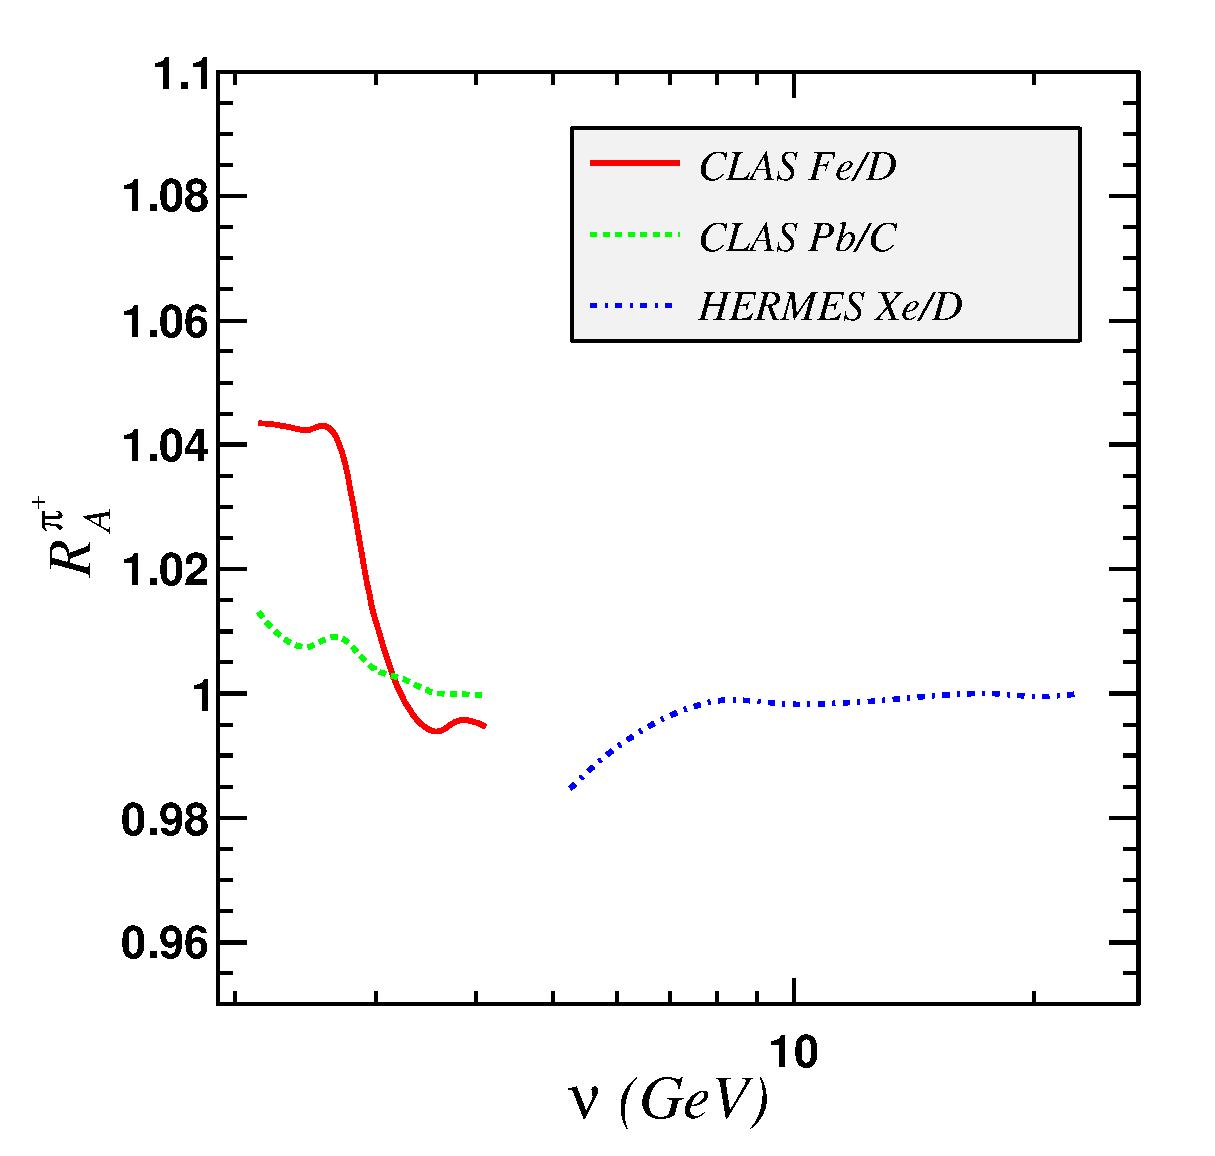
\includegraphics{fig/Ratio_FM_Nu.eps} }
\resizebox{0.32\textwidth}{!}{
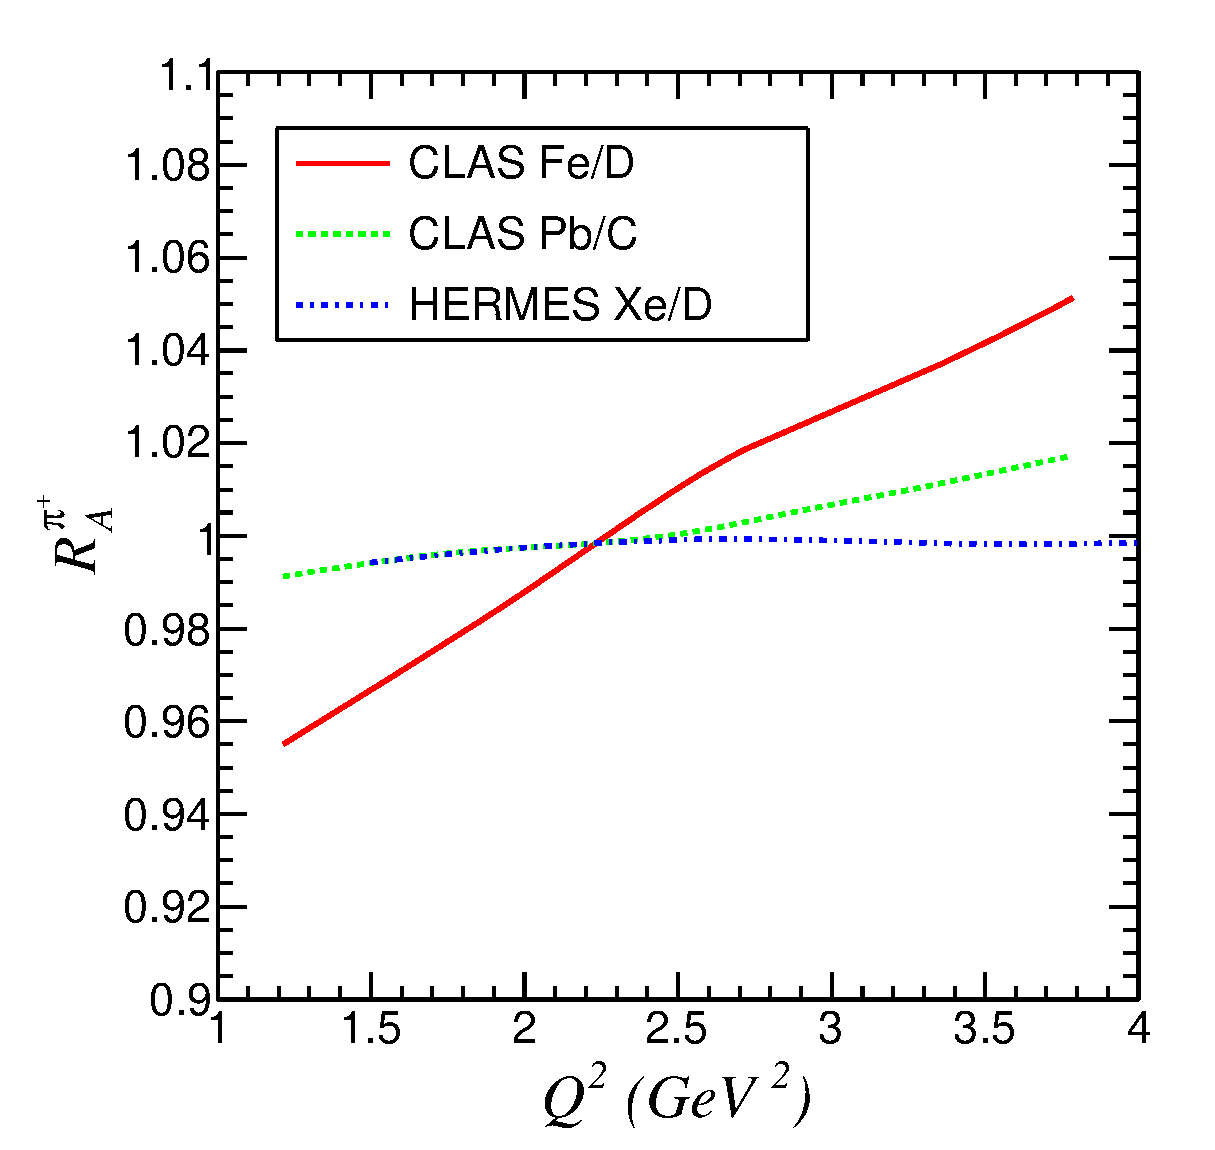
\includegraphics{fig/Ratio_FM_Q2.eps} }
\resizebox{0.32\textwidth}{!}{
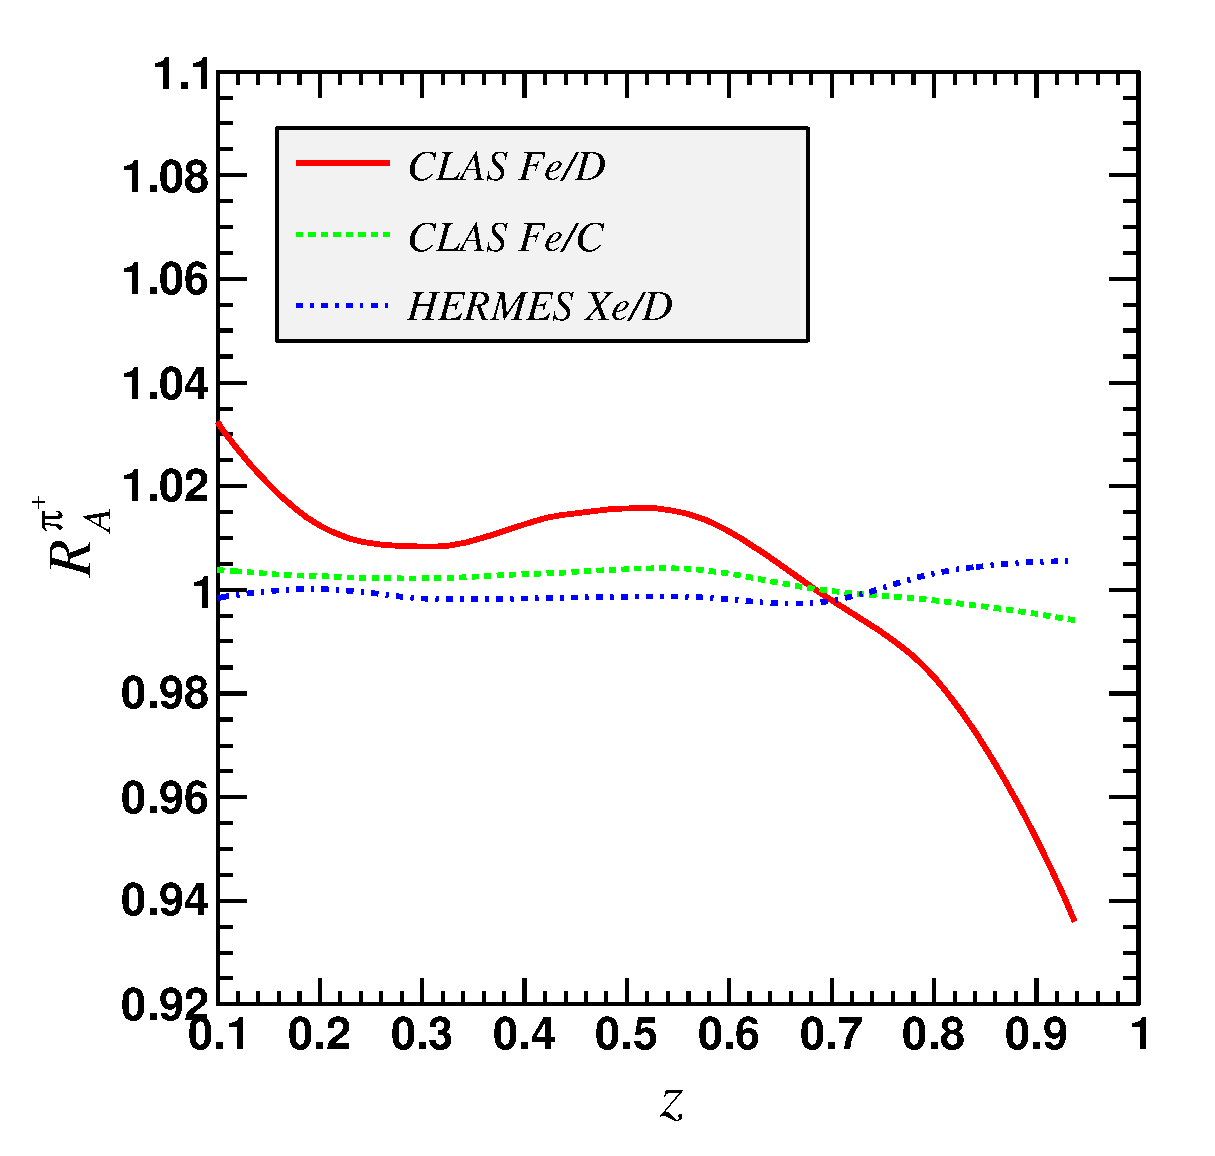
\includegraphics{fig/Ratio_FM_Z.eps} }
\caption {Multiplicity ratio as a function of $\nu$, $Q^2$, and $z$ calculated based only on Fermi motion effects. The red dotted line is for CLAS Fe/D, the green dashed for Fe/C and the blue dot-dashed line for HERMES Xe/D.}
\label{fig:FM-R}
\end{figure*}

\begin{figure*}[tbp]
\centering
\resizebox{0.33\textwidth}{!}{
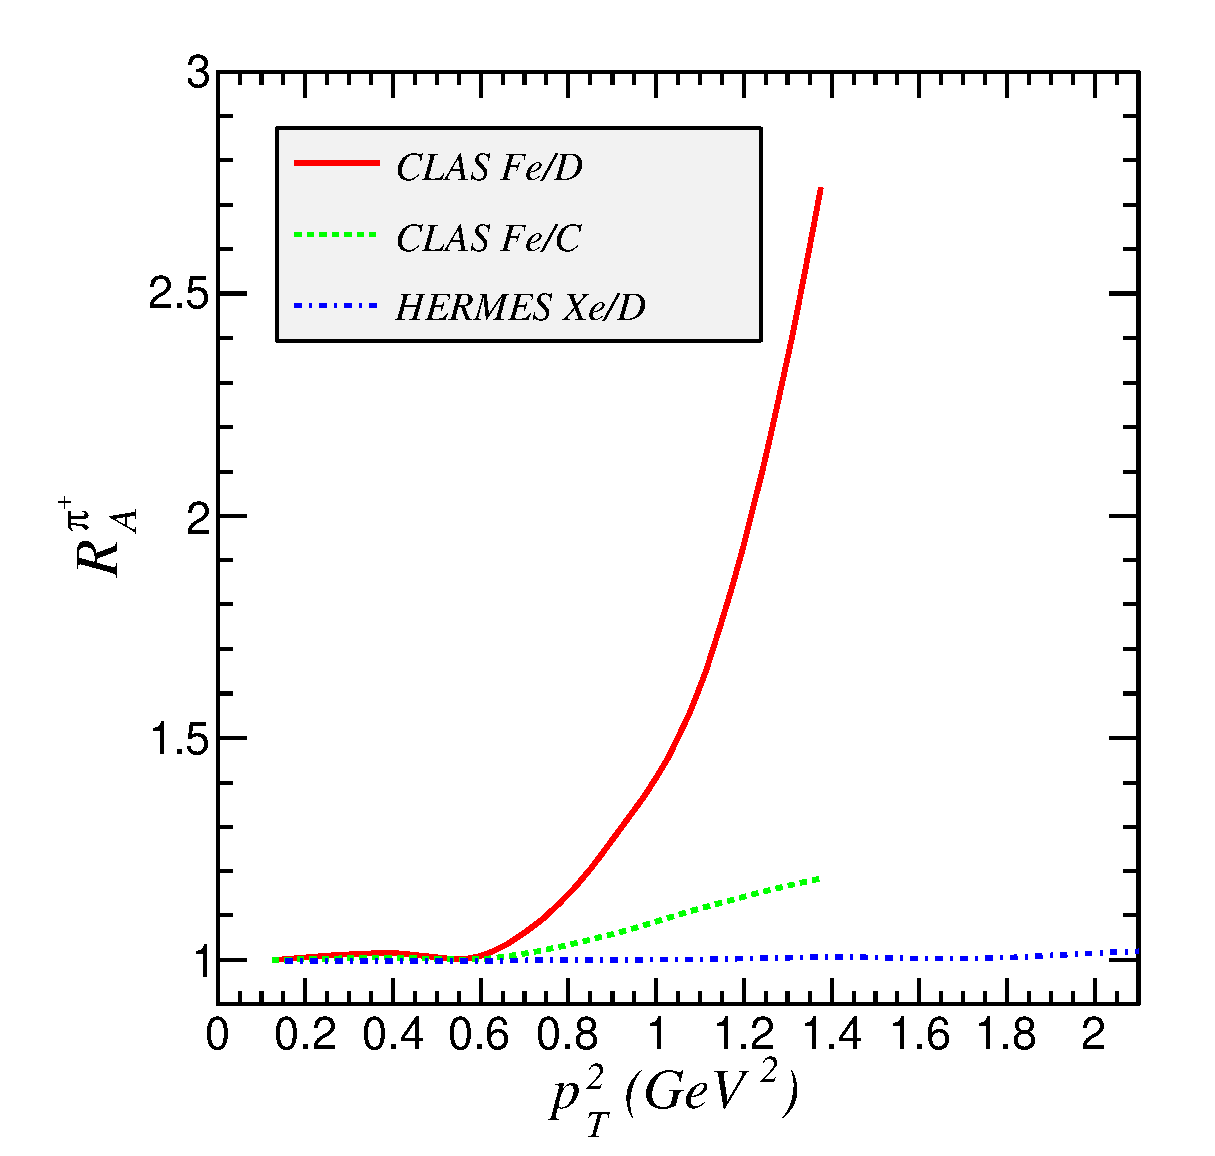
\includegraphics{fig/Ratio_FM_Pts-2.eps} }
\resizebox{0.33\textwidth}{!}{
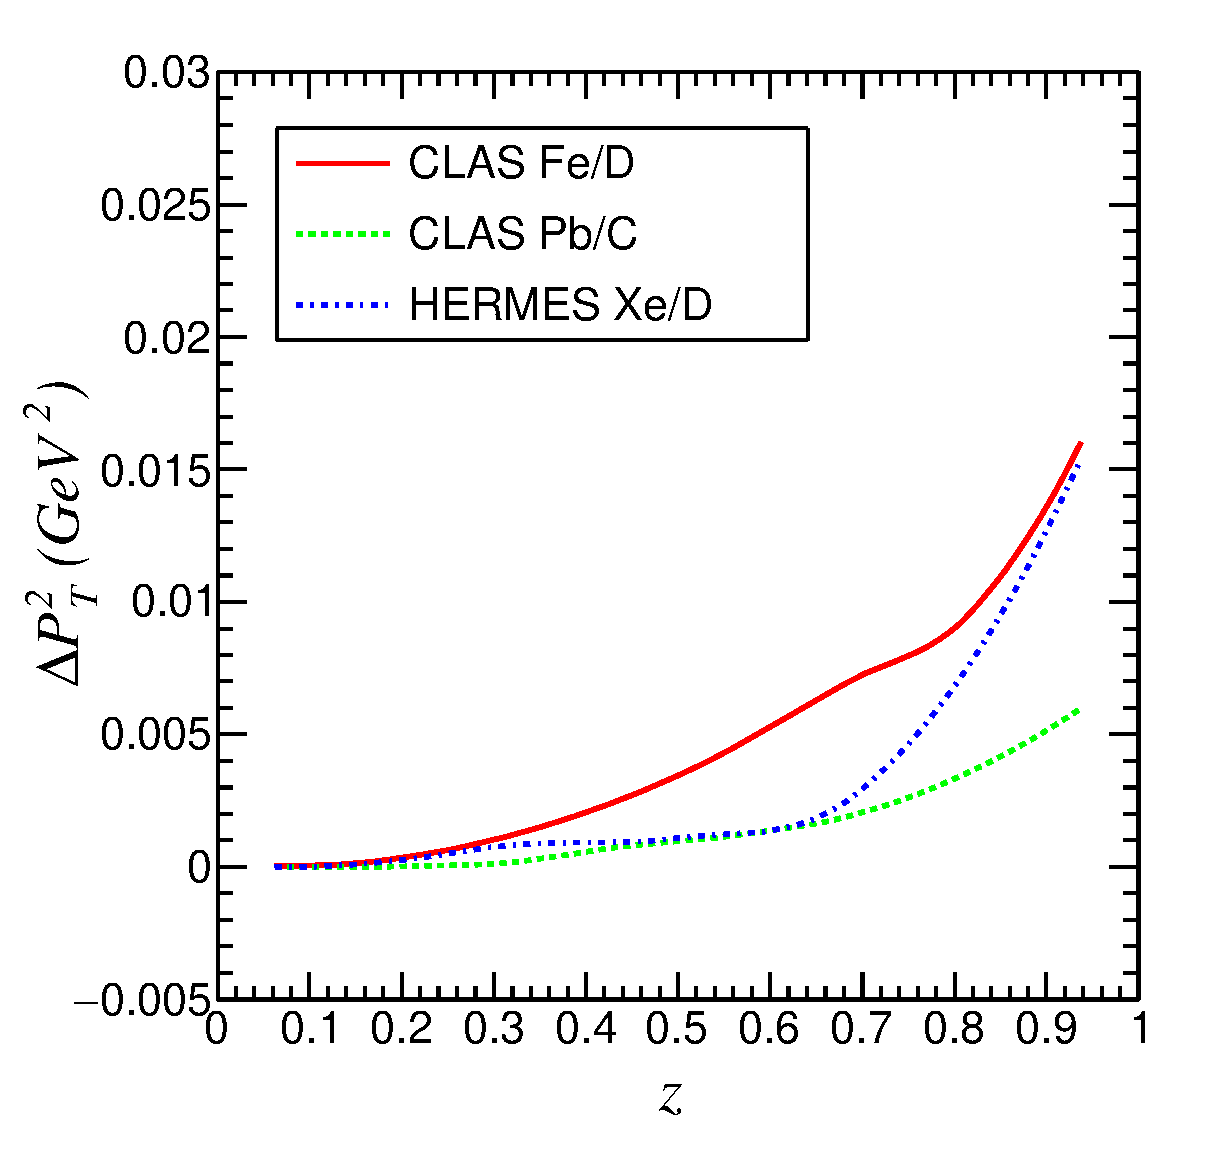
\includegraphics{fig/DPts_FM_Z.eps} }
\caption {Multiplicity ratio as a function of $p_T^2$ (left panel) and transverse momentum broadening as a function of $z$ (right panel) calculated based only on Fermi motion effects. 
The red dotted line is for CLAS Fe/D, the green dashed 
for Fe/C and the blue dot-dashed line for HERMES Xe/D.
{\bf [AA] Raphael, it may be nice always use Pb/C (rather than Fe/C as it happens in 2 of these figures ($R_A$ vs. $P_T^2$ and vs. $z$.)}
}
\label{fig:FM-Rpt-DPtz}
\end{figure*}


\section{Fermi Motion}

Fermi momentum, {\em i.e.}, the momentum carried by nucleons relative to the nucleus in which they are bound, can lead to hadron attenuation and transverse momentum broadening and mimick the effects due to in-medium parton propagation.
Indeed, we expect that Fermi motion will affect the hadron multiplicity because of the change in center of mass energy of the electron-nucleon interaction it create. 
With large numbers of events these effects should mostly cancel because higher than average electron-nucleon energies will compensate lower than average ones, but it is important to evaluate the residual effects with our MC simulation. 

The typical Fermi momentum is of the order of a few hundreds of MeV, and is therefore expected to have limited impact on multiplicities ratios measured at the HERMES experiment (electron or positron beam of 27.5~GeV). However, as we shall see, its impact on ratios from the CLAS experiments at JLab, for which preliminary data with a 5~GeV electron beam are available~\cite{Brooks:2009xg,DupreQNP}), is typically non negligible. 
Moreover, due to the rapidly decreasing $p_T$ spectrum, it is unclear how effects on $i\Delta p_T^2$ are reduced at high energy and Fermi motion can affect even HERMES data for this observable.

In absence of Fermi motion all nucleons are consiered at rest in the nucleus frame. 
Fermi motion is therefore implemented in our MC by assigning the target nucleon an initial 3-momentum before running Pythia. The nucleon three momenta are then distributed on the full solid angle with a distribution in magnitude taken from the parametrization by Ciofi degli Atti and Simula \cite{CiofidegliAtti:1995qe}.
In our model, nucleons are taken to be on-shell, which seem an reasonable simplification for the relatively small values of $x$ we explore.

In Figure~\ref{fig:FM-R} we show the results of the described MC simulation on the hadron multiplcity ratio $R_M$. No sizable effects is visible as a function of the inclusive variables $x$ and $\nu$ for HERMES energy, but at CLAS energy the multiplicity ratio observables are affected at a few percent level. Similarly, as a function of the semi-inclusive variable $z$, we obtain a small (up to 2\%) effect in the factorization region ($0.3 \lesssim z \lesssim0.8$). 

The effects of Fermi motion on the hadrons $p_T$ spectrum, which are expected to be the largest, are shown in figure~\ref{fig:FM-Rpt-DPtz}. In the case of the multiplicity ratio $R_M$ as a function of $p_T^2$ (left panel), and for the 
hadron $p_T$-broadening $\Delta p_T^2$ as a function of $z$.
At HERMES energy no sizable effect is visible on $R_M$. However, at CLAS energy a very large effect is observed. This is particularly problematic because this signal can mimic the Cronin effect due to in-medium multiple soft scattering~\cite{Kopeliovich:2003py}, and limit the interpretability of CLAS measurements in terms of medium modification of parton propagation.
Similarly to the effects on the $p_T$ spectrum, FM generates an initial state transverse momentum broadening. This however can be expected to be less sensitive to energy variations because in $\Delta P_T^2$ the effect is relative to the average transverse momenta in which proportionnaly varies less than the beam energy.
Indeed, the result of our simulation at HERMES energy indicates a small but clear FM effect, which corresponds to 5--10\% of the total observed broadening. The effect grows with $z$ as should be expected, because the fraction of energy carried by the hadron is proportionnal to the fraction of transverse momentum transferred from the parton to the hadron. 

In order to reduce FM effects for all observables at CLAS energy (and eventually for future experiments) but not unduly cancel the effects from final state interactions with the medium, we propose to utilize Carbon (instead of Deuteron) as the reference nucleus in the denominator of the multiplicity ratio and for transverse momentum broadening. Indeed, the average nucleon momentum vary very little from Carbon to Lead \cite{CiofidegliAtti:1995qe} making the Fermi motion effects similar and therefore cancel them for the $R_M$ and $\Delta P_T^2$ observables. The green dotted lines in Figures \ref{fig:FM-R} and \ref{fig:FM-Rpt-DPtz} show a significant reduction of FM effects in the multiplicity ratio using this option. In particular, the FM effects are brought below the 0.5\% level in the transverse momentum broadening.


\section{Parton radiative energy loss}
\label{sec:qweights}

We describe the medium-induced radiative energy loss of scattered partons in the quenching weight formalism of Armesto, Salgado and Wiedemann \cite{Salgado:2002cd,Salgado:2003gb,Armesto:2003jh}. In the ASW model, the medium is modelled as a collection of colored static scattering centers, with a given density distribution along the parton trajectory, and it is assumed that the parton interacts via multiple soft scatterings. Recoil effects are neglected, which amounts to neglecting the so-called elastic energy loss. 
The medium is then effectively described by the transport coefficient $\hat
q$, which carachterizes the amount of transverse momentum gained by the scattered parton per unit path length in the medium, or, rather, by the radiated gluons carachteristic energy in a medium of length $L$:
\begin{align}
  \omega_c & = \frac12 \hat q L^2 \ .
\end{align}
The ASW model was originally based on the BDMPS-Z path integral formulation formulation of the energy loss problem, assuming a medium of infinite length. Finite length effects, which are very important in the case of cold nuclear matter, have then been introduced by properly cutting off large angle gluon radiation. This cutoff is controlled by
\begin{align}
  R = \omega_C L \ ,   
\end{align}
which accounts for thr fact that the transverse momentum of a radiated gluon cannot be larger than its energy. The end product is a so-called ``quenching weight'', 
\begin{align}
  \PP(\epsilon) = p(\epsilon) + p_0 \delta(\epsilon) 
\end{align}
which encodes the probability distribution for energy loss $\epsilon$ in a medium of length $L$ and transport coefficeint $\hat q$. Here, $p(\epsilon)$ its continuous part and $p_0$ the probability that the parton traverses the medium with no reinteractions, and tehrefore no energy loss. {\bf [AA] Add discussion of ``death on arrival'' here? Or later when we give more details?}

\begin{figure}[tbp]
  \centering
  \resizebox{0.45\textwidth}{!}{
    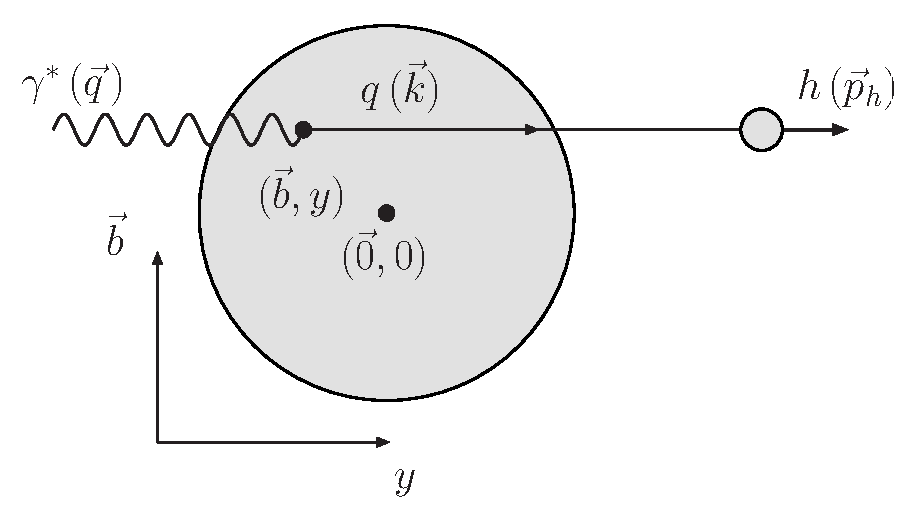
\includegraphics{fig/DIS-geom.eps} }
  \caption{Geometry of hadron production in nDIS in the nucleus 
    target rest frame. The particles 3-momenta are in parentheses.}
  \label{fig:DISgeom}
\end{figure}

The ASW quenching weight is computed for a static and uniform 
medium with characteristic gluon energy $\bar\omega_c$ and size parameter 
$\bar R$. However, a quark traveling thorugh either an expanding hot medium such as the Quark Gluon Plasms, or a cold nuclear matter medium such as the target nucleus in a DIS experiment, experiences a decreasing medium density along its path. This requires a phenomenological treatment of non uniform density media \cite{Salgado:2003gb,Dainese:2004te,Accardi:2007in}.

In the DIS case, following \cite{Accardi:2007in}, the nuclear geometry can be approximated by the nuclear positive charge density distribution 
$\rho_A(\vec x)$ (from~\cite{DeJager:1987qc}), where $\vec x=(\vec b,y)$, $y$ 
is the coordinate along the direction of the virtual photon, $\vec b$ its 
impact parameter, and the center of the nucleus lies at $\vec x = (\vec 0,0)$ as pictured in Fig.~\ref{fig:DISgeom}.  
%
The nucleus density is static but non-uniform. We can then assume the average tarnsverse momentum transfer to be proportional to the parton's mean free path $\lambda = (\sigma \rho_A)^{-1}$, where $\sigma$ is the parton's cross-section, assumed fixed and independent of the atomic number. This is equivalent to assuming that the transport coefficient is proportional to the mean free pasth, $\qhat \propto \lambda$, and we can define a 
position-dependent transport coefficient,
\begin{align}
  \qhat_A (\vec b,y) = \frac{\qhat_0}{\rho_{0}} \rho_A(\vec b,y) \ ,
 \label{eq:qhatby}
\end{align}
where $\qhat_0 = \qhat_{\bar A}(0,0)$ is the transport coefficient at the 
center of a reference nucleus of atomic number $\bar A$, and $\rho_{0} = 
\rho_{\bar A}(0,0)$.

Next, we consider a quark struck at $(\vec b,y)$ which propagates in the nucleus along the $y$ direction. We define its average path-length $\bar L_A$:
\begin{align}
  \bar L_A(\vec b,y) = 2 \frac{\int_y^\infty dz\, (z-y)\rho_A(\vec b,z)}
    {\int_y^\infty dz\, \rho_A(\vec b,z)} 
\end{align}
the average nuclear density $\bar\rho_A$ seen by the quark:
\begin{align}
  \bar\rho_A(\vec b,y) =  \frac{\int_y^\infty dz\, \rho_A(\vec b,z)}{\bar 
  L_A(\vec b,y)} \ ,
\end{align}
and, from Eq.~\eqref{eq:qhatby}, the average transport coefficient experienced 
by the quark:
\begin{align}
  \bar\qhat_A (\vec b,y) = \frac{\qhat_0}{\rho_0} \bar\rho_A(\vec b,y) \ .
\end{align}
For a uniform hard-sphere nuclear density $\rho_A(r) = \rho_0 \theta(R_A-r)$, 
the above definitions give $\bar L_A = R_A - y$, $\bar\rho_A = \rho_0$, and 
$\bar\qhat_A = \qhat_0$ as it should be.

According to Eqs.~\eqref{eq:omegac}-\eqref{eq:R}, we can define the average 
characteristic gluon energy $\bar\omega_c$ and size parameter $\bar R$ as 
follows:
\begin{align}
  \bar\omega_c(\vec b,y)& \equiv \frac{1}{2} \bar\qhat_A(\vec b,y) 
    \bar L_A^2(\vec b,y) 
    = \int_y^\infty dz\, (z-y)\qhat_A(\vec b,z) 
  \label{eq:omegacbar} \\
  \bar R(\vec b,y) & \equiv \bar\omega_c(\vec b,y) \bar L_A(\vec b,y) 
    = \frac{2 \bar\omega_C^2(\vec b,y)}{\int_y^\infty dz\,
    \qhat_A(\vec b,z)} \ , 
  \label{eq:Rbar}
\end{align}
where in the last equalities there is no explicit dependence on the definition 
of the average medium length $\bar L_A$. These equations correspond to Eqs.~(8) 
and (10) of Ref.~\cite{Dainese:2004te}, that treated the case of hot nuclear matter. Note that these quantities depend on only one parameter, $\qhat_0$, analog of $k$ in the cited reference. Finally, one can easily see that
\begin{align}
  \bar\qhat_A(\vec b,y) = \frac{2}{\bar L_A^2(\vec b,y)} \int_y^\infty dz\,
    (z-y)\qhat_A(\vec b,z) \ ,
\end{align}
as discussed by Salgado and Wiedemann \cite{Salgado:2003gb}. In that paper, it was proven that one can approximate the quenching weight for a dynamically expanding medium with the quenching weight for an equivalent static (and uniform) medium characterized by the average $\bar\qhat_A$. However, the natural parameters of the quenching weight are the gluon characteristic energy and the size parameter. Hence, the obtained scaling law is more properly expressed by saying that the equivalent static and uniform medium is characterized by the average $\bar \omega_c$ and $\bar R$ \cite{Dainese:2004te}. In nuclear DIS we have, however, a static but non-uniform medium. For a propagating parton, the spatial non-uniformity is equivalent to a time-evolution of the medium. Therefore, as an {\it ansatz}, we may generalize the SW scaling law to the case of the static but non-uniform medium encountered in nDIS, and use Eqs.~\eqref{eq:omegacbar}-\eqref{eq:Rbar} in the quenching weight evaluation. This {\it ansatz} will need to be better substantiated in the future. In particular, we note that the SW scaling law has only been established only for $\bar R \gtrsim 100$. In applications to nDIS, however, $\qhat_A < 1\ \text{GeV$^2$/fm}$ and one 
has typically pretty low values of $\bar R$ with a significant part of the 
events below this limit. Nonetheless, those events have small quenching weights and do not contribute much to the nuclear effects, so that we feel it appropriate for the purposes of this paper to extend the scaling law to the nuclear DIS case.


\section{Parton transverse momentum broadening}
\label{sec:ptbroad}

Along its path the parton can rescatter in the nuclear medium, not only radiating gluons (thereby loosing energy) but also acquiring some additional transverse momentum, resulting on average in a broadening of the final transverse momentum of the produced hadrons compared to scattering on proton or deuteron targets. Measuring this transverse momentum broadening  
is a way to access information on hadronization independently of the 
attenuation caused by energy loss. Therefore a coherent explanation of both attenuation and transverse momentum observations by our model is an important objective to demonstrate the completeness of the model.
 
Unlike for parton energy loss, no readily utilizable probability distribution is presently available in literature for the case of medium induced parton transverse momentum broadening. We therefore investigate a few different ways to implement this effect in our simulation consistently with the ASW model of parton energy loss. The 2 most sofisticated ones are an {\it Ansatz} for unintegrated ASW quenching weights, which produces a probability distribution for the average emission angle of gluon radiation and is suitable for an event-by-event transverse momentum generation. We then compare this with a more basic models which makes direct use of the transport parameter $\qhat$, and with a baseline simulation where no transverse momentum is added to the parton propagating in the nucleus.  

{\bf 
[RD] We should define the names for each scenarios used in the figures here? Or is it clear enough?

[AA] We definitely SHOULD find better names -- but I am reputedly bad at this. I'll try my best, though.
}

\subsection{Angular dependent ASW quenching weights}
\label{sec:angular_quenching}

The calculation of the probability distribution in polar angle of the radiated energy requires defining the gluon energy distribution outside a polar angle $\Theta$, Eq.(5.2) of \cite{Salgado:2003gb}, and inserting this in the Mellin transform (3.2)-(3.3) of \cite{Salgado:2003gb}. Since this calculation has not yet been performed, here we resort to an {\it Ansatz}. The average energy loss outside an azimuthal angle $\Theta$ can be computed in the ASW formalism as
\begin{align}
  \vev{\Delta E}(\chi > \bar\chi) = \int d\epsilon \epsilon 
    \big[ \PP(\epsilon;\omega_c,R) - \PP(\epsilon;\omega_c,\chi^2 R) \big] 
\end{align}
where $\chi = \sin \Theta$ and $\Theta$ is the radiated energy angle with 
respect to the parton's 3-momentum. Then the angular distribution of the 
average radiated energy is  
\begin{align}
  \frac{d\vev{\Delta E}}{d\chi} = \int d\epsilon \epsilon 
    \frac{d}{d\chi}\PP(\epsilon;\omega_c,\chi^2 R) \ . 
\end{align}
This allows to define a quenching weight for the {\it average} energy 
deposition at angle $\chi$:
\begin{align}
  \EE(\epsilon,\chi;\omega_c,R) = \frac{d\vev{\Delta E}}{d\epsilon d\chi} 
    = \epsilon\,\frac{d}{d\chi}\PP(\epsilon;\omega_c,\chi^2 R) \ . 
\end{align}
The total energy loss with no angular restrictions except the general one, 
$\Theta\leq \pi/2$, is obtained by definition as:
\begin{align}
  \vev{\Delta E} = \int d\epsilon \int_0^1 d\chi\, 
    \EE(\epsilon,\chi;\omega_c,R) \ .
\label{eq:integrated_ang_qw}
\end{align} 


\subsection{ASW transverse momentum}
\label{sec:angularASW}

A calculation of the propagating parton transverse momentum spectrum in the path-integral formalism utilized to calculate the ASW quenching weights involves cutting the quark line instead of the radiated gluon line. This would describe the quark transverse dynamics including the elastic scattering on the colored scattering centres in the medium as well as respecting transverse momentum conservation in the radiation process. 

This calculation is unfortunately not presently available within the ASW formalism, therefore as an approximation we neglect the transverse momentum gained in the elastic scattering, and require the quark to only balance the transverse momentum of the radiated gluons. This is a rough approximation, but suitable for the exploratory nature of this paper, which purports among other things to determine the sensitivity of nuclear SIDIS observables to the dynamics of color charge propagation in cold nuclear matter. Furthermore, it will be corrected (to some extent) in the next subsection.

We then use the quenching weight $\cal E$, suitably normalized, to generate event-by-event both the radiated gluon energy $\epsilon$ and its emission polar angle $\Theta = \sin^{-1} \chi$. With a uniformly azimuthal angle $\phi$ we then construct 4-momentum of the gluon and, by energy-momentum conservation, that of the quark.  


\subsection{BDMPS mean}

Next, we consider the relationship between $\vev{k_T^2}$ and $\vev{\epsilon}$, 
established in the seminal paper \cite{Baier:1996sk} by Baier, Dokshitzer, Mueller, Peign\'e and Schiff (BDMPS),
\begin{align}
  \vev{k_T^2} = \frac{8}{\alpha_s N_c} \frac{\vev{\Delta E}}{L} \ ,
 \label{eq:avepsmt_main}
\end{align}
which within the assumptions of the calculation is valid for finite-length matter, cold or hot, and is independent of the parton flavor. It is also important to note that this relationship is independent of the details of the dynamics of the individual parton scatterings.

The {\it Ansatz} here consists in extending \eqref{eq:avepsmt_main} to the differential level:
\begin{align}
  \frac{d\vev{k_T^2}}{d\epsilon d\chi} & = \frac{8}{\alpha_s N_c L}
    \ \frac{d\vev{\Delta E}}{d\epsilon d\chi} \ .
\label{eq:enangdist}
\end{align}
Thus one can define a probability distribution in $\epsilon$ and $\chi$, and use it to generate the 4-momentum $k$ of the parton up to a random azimuthal angle $\phi$. It is important to note that this formula takes properly into account the coupled effects of elastic scattering and gluon radiation on the parton transverse momentum, which were neglected in the approximation proposed in Section~\ref{sec:angularASW}.

In our Monte-Carlo simulation, $L$ is replaced by $\bar L$ in order to account for the realistic profile of the nuclei. Furthermore, and more importantly, we use the ASW angular dependent
\begin{align}
  \frac{d\vev{\Delta E}}{d\epsilon d\chi} = \EE(\epsilon,\chi;\omega_c,R)  
\end{align}
derived in Section~\ref{sec:angular_quenching}. Note that this introduces a dependence on the medium size through the $R$ parameter, that accounts for large angle radiation kinematic constraints neglected in the pioneering BDMPS paper.

\subsection{Naive $\qhat$}

By definition $\qhat$ is the mean transverse momentum square gained by per unit pathlength in the medium. It is therefore possible to increase the transverse momentum of each parton by $(\qhat \bar L)^{1/2}$, with a randomly generated azimuthal angle. The main advantage of this {\it Ansatz} is to insure that the input parameter $\qhat$ corresponds more directly to the quark transverse momentum broadening that can be inferred from the measured hadron transverse broadening. Yet, unlike the previous two, this {\it Ansatz} completely disconnects the longitudinal quenching from the transverse momentum acquired by the parton, and the results should therefore be interpreted with care.


\subsection{No transverse momentum}

By keeping the initial direction of the parton, i.e. no transverse momentum, one can study other sources of medium modifications of the hadron transverse momentum. The FM effects were already discussed, and found to be largely (but not wholly) negligible at HERMES energy. However, even pure longitudinal quenching of a parton affects the hadron $p_T$ spectrum, because of the reduced energy available to the hadronization process. This effect is often overlooked in literature assuming quenching is small. However, for a correct interpretation of experimental data it is important to quantify the impact of these effects.


\section{Monte Carlo implementation and hadronization}
\label{sec:MC_implementation}

{\bf [AA] QUESTION: should we have only one MC implementation discussion here
for both energy loss and broadening, or would you prefer one in each of the preceding sections?}\\


\noindent{\bf 
TO DO: 
\begin{itemize}
  \item Details of random radiation generation, quark momentum after gluon radiation
  \item What happens to the radiated gluons
  \item Energy-momentum conservation (implementation and effects)
  \item How to treat negative probability (rescaling, other?)
  \item Did we consider elastic energy loss at all? 
  \item How to treast events with $R<1$ 
  \item Specifics of the broadening models
  \item ...
  \item Discuss the hadronization model used (Lund as in JETSET), stress some of the differences w.r.t. using Fragmentation Functions.
  \item ...
\end{itemize}
}


{\color{red} --------- EDITED DOWN TO HERE [AA] -----------}


\section{Comparison to HERMES data}

\ \ \ \ 
{\bf [AA] Questions: Should we discuss in more details the implications of the 
kinematical cuts used by HERMES ?}

{\bf [AA] It may be interesting be to add a comparison figure to the analytical calcualtion - in principle I have code for that, and if we still have energy when we are done with the rest of the paper, I might give it a thought.}


\begin{figure}[tbp]
  \centering
\resizebox{0.45\textwidth}{!}{
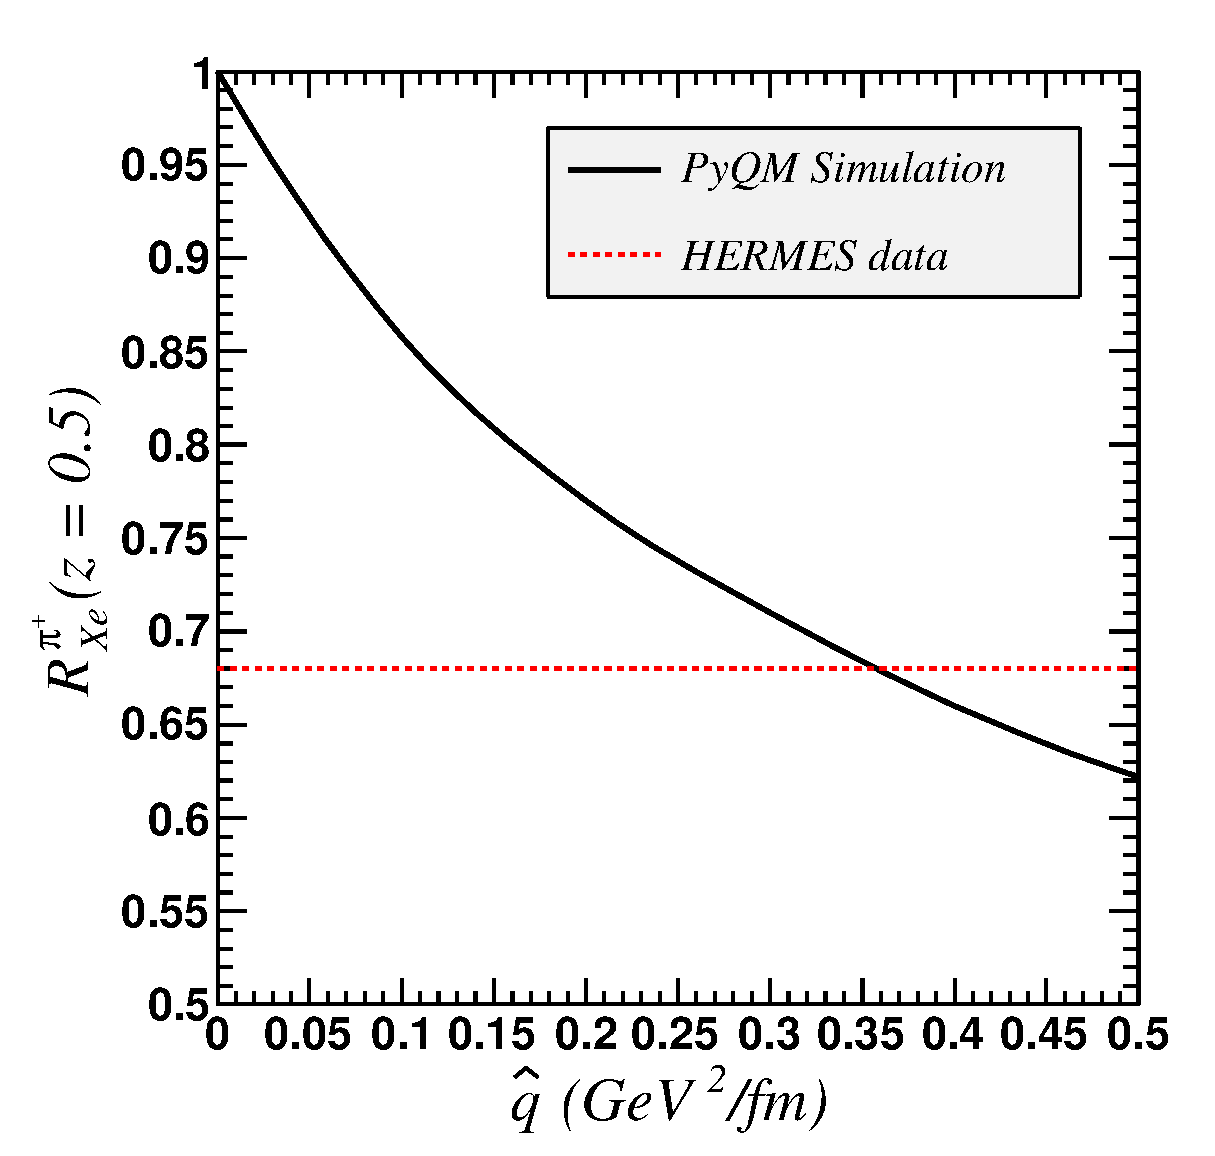
\includegraphics{fig/Ratio_HP3_qhat.eps} 
}
\caption {Multiplicity ratio of xenon for $z = 0.5$ as a function of $\qhat$. 
The red dashed line indicates the experimental value measured by HERMES~%
\cite{Airapetian:2007vu}.}
\label{fig:qhat}
\end{figure}

...........

We use the same kinematical cuts adopted in the HERMES analysis, namely, $\nu > 6$ GeV and $2 < P_\pi < 15$~GeV \cite{Airapetian:2007vu,Airapetian:2009jy}.

..............


\subsection{Extraction of $\qhat$}

The parameters $\bar\omega_c$ and $\bar R$ used in the quenching weights 
calculation depend only of one free parameter, $\qhat_0$. To determine its 
value, we need to calibrate our simulation. Since we have several scenarios 
for the transverse momentum implementation, it seems more precise to use the 
attenuation observable for this calibration. We show in figure~\ref{fig:qhat} 
the multiplicity ratio of xenon at $z=0.5$ as function of $\qhat$. The MC 
implementation of the transverse momentum broadening gives a result of $\qhat_0 
= 0.36$ GeV$^2$/fm to match HERMES data. We will use this value for all 
scenarios, which might reduce their capability to describe the data. However, 
it will allow to compare the effect of the different options on the same basis.

Most models and comparison to data give a $\qhat$ between 0.05 and 0.6~GeV$^2$/fm in cold nuclear matter~\cite{Accardi:2009qv}. Our value appears to be relatively large in this range but still reasonable. This result is in particular comparable to Arleo's 
result: $\qhat = 0.14$ GeV$^2$/fm~\cite{Arleo:2002ph,Arleo:2003jz}. Possible 
reasons for this discrepancy are that Arleo's computation is done at fixed 
length $\bar L_A = (3/4) R_A$, and does not include finite size corrections 
($\bar R = \infty$) and that Arleo uses $\alpha_s=0.5$ and ASW use 
$\alpha_s=0.3$ in their quenching weight computation. An extraction of the transport coefficient that includes the nuclear geometry and finite length effects as in this paper, but otherwise relies on an analytical calculation as in teh rpevious paper, was first obtained by Accardi \cite{Accardi:2007in} and later updated in Ref.~\cite{Accardi:2009qv}, resulting in a five times larger vale of $\hat q = 0.6$ GeV$^2$/fm. This shows how realistic geometry effects affect the quantitative extraction of the transport coefficient, as well as the relevance of a MC decription of hadronization that again reduces that value. 

{\bf [RD] do we have other values to compare with? [AA] Maybe these 2 examples are enough, showing the importance of geometry and MC treatment. However some rewrighting is in order.}


\begin{figure}[tbp]
  \centering
\resizebox{0.45\textwidth}{!}{
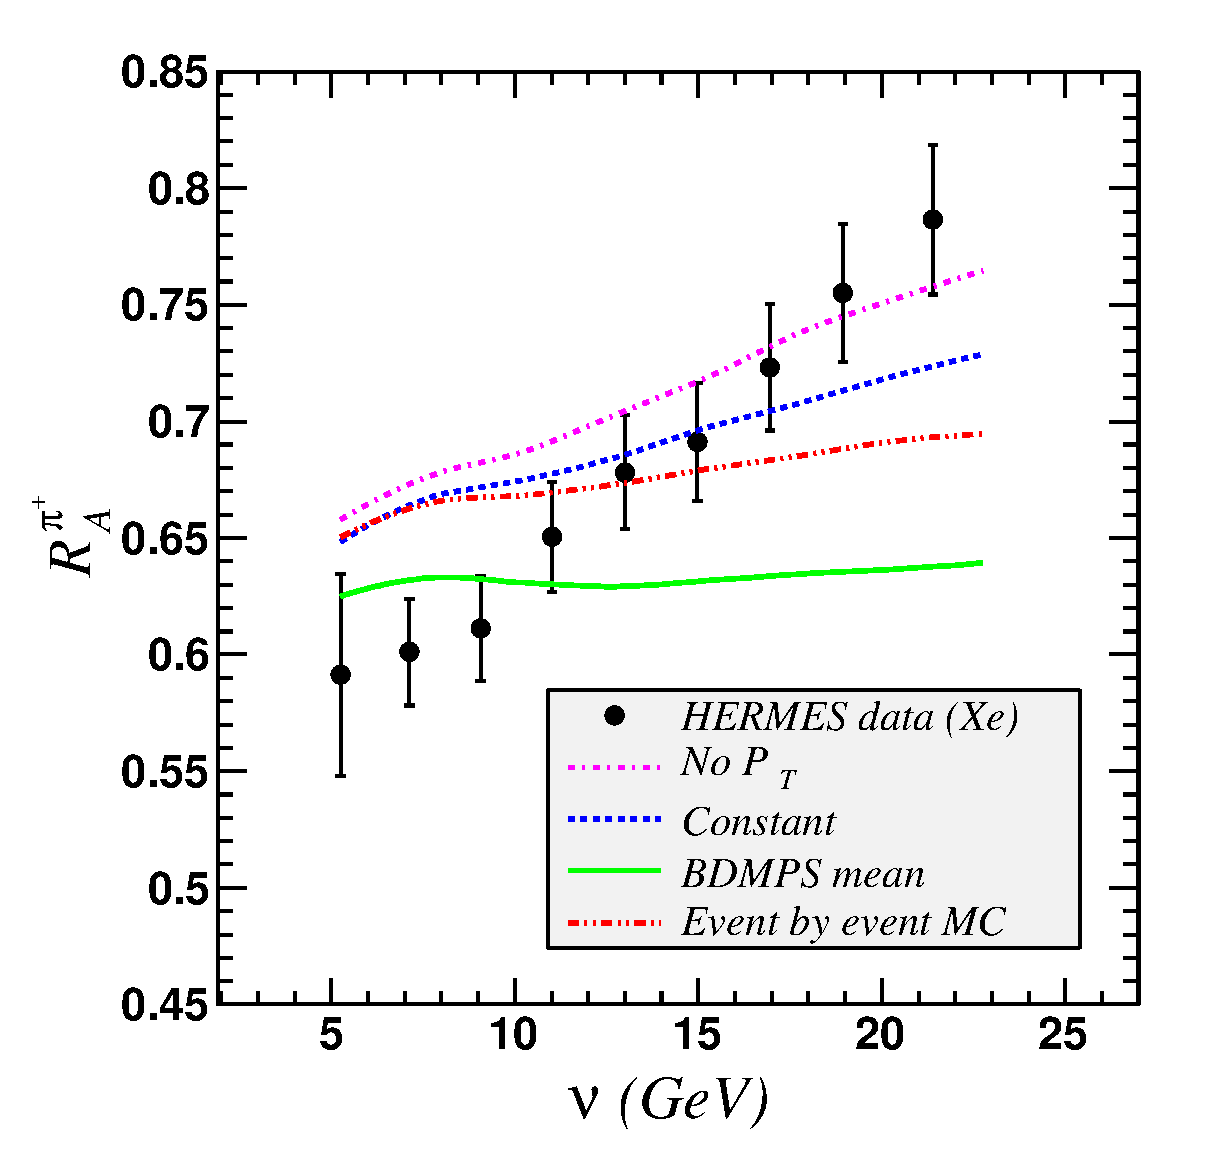
\includegraphics{fig/R_Nu_CompPt.eps} }
\caption {Multiplicity ratio of xenon as a function of $\nu$. HERMES data~%
\cite{Airapetian:2011jp} (points) are compared with Monte-Carlo simulation 
(lines) for different transverse momentum broadening implementations (see 
section~\ref{sec:ptbroad}).}
\label{fig:PtC-Rnu}
\end{figure}


\subsection{Hadron attenuation}

Using the calibrated MC, we can now describe our observables in more detail. 
First, figure~\ref{fig:PtC-Rnu} shows our result for the multiplicity 
ratio as a function of $\nu$ for the different options of transverse momentum. 
The result shows that transverse momentum options have some impact on the 
observed attenuation. This effect is due to the reduction of the center of mass 
energy when we enhance the transverse momentum of the parton. Indeed, when 
applying transverse momentum, we conserve parton energy in the lab frame (the 
rest frame of the nuclei) which is the most relevant for hadronization studies. 
This result also shows that different implementations of $p_T$ broadening can 
lead to different slopes as function of $\nu$. This is particularly important 
and shows that a proper implementation of transverse momentum broadening is 
mandatory to describe completely and coherently the data. However, in all 
cases the slope seems to be too low to describe properly the data from HERMES~%
\cite{Airapetian:2011jp}. This problem can be either directly linked to the 
calculation or to some of the identified weakness of our implementation, in 
particular the lack of treatment of the radiated energy or an incorrect parton 
spectrum produced by Pythia.

\begin{figure}[tbp]
  \centering
\resizebox{0.45\textwidth}{!}{
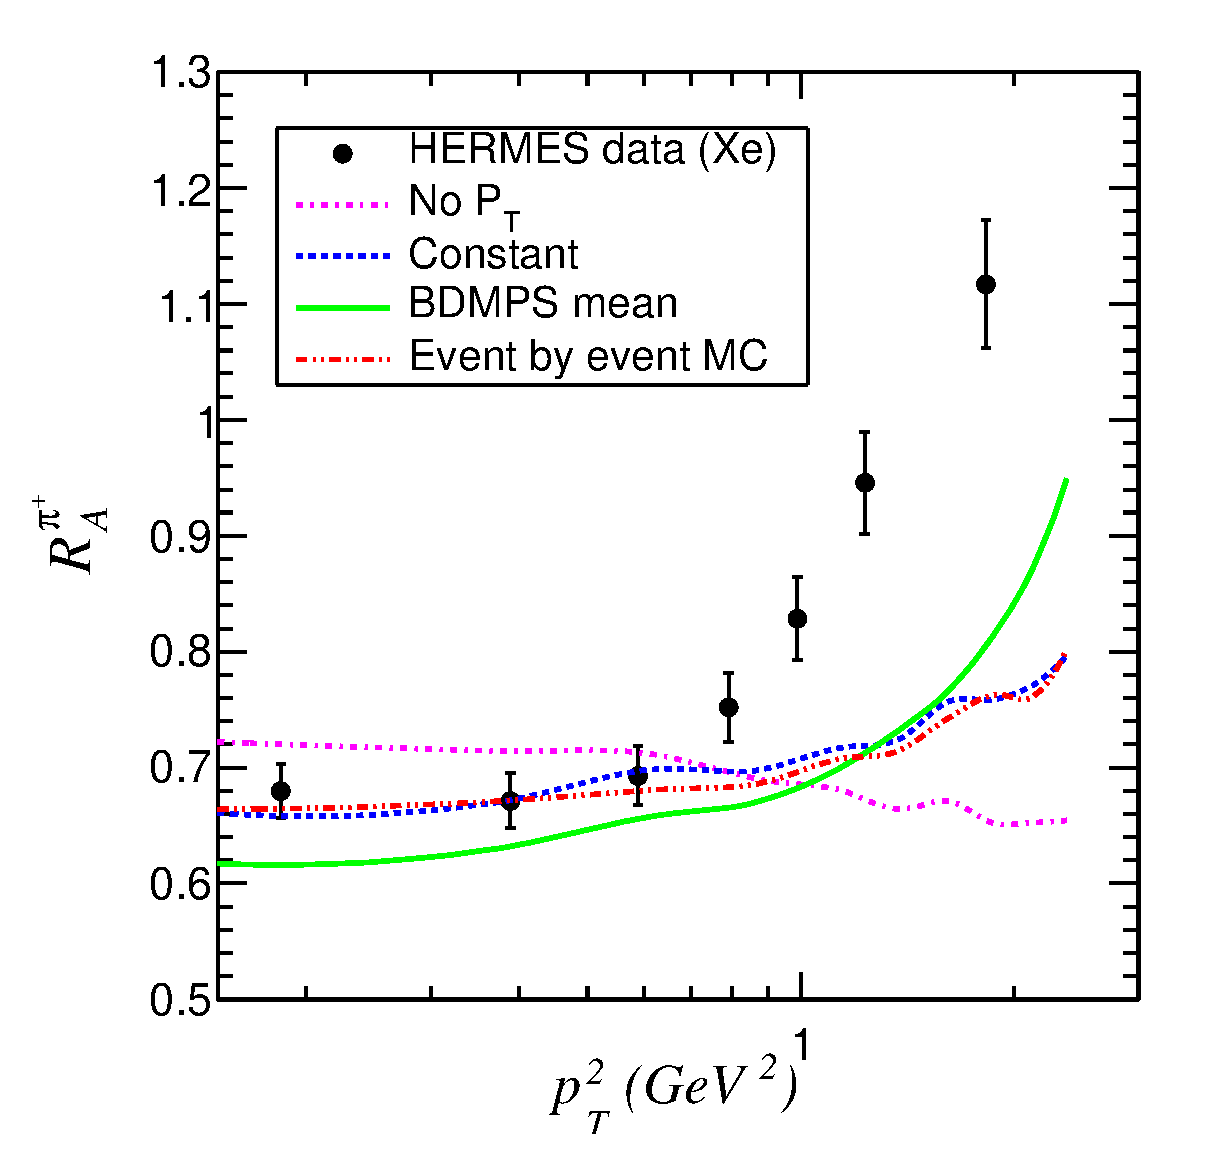
\includegraphics{fig/R_Pts_CompPt.eps} }
\caption {Multiplicity ratio of xenon as a function of $p_T^2$. HERMES data~%
\cite{Airapetian:2011jp} (points) are compared with Monte-Carlo simulation 
(lines) for different transverse momentum broadening implementations (see 
section~\ref{sec:ptbroad}).}
\label{fig:PtC-RPts}
\end{figure}


\subsection{Transverse momentum dependent observables}

An important test for the transverse momentum implementation is the 
reproduction of the so called Cronin effect, corresponding to an important 
increase of the multiplicity ratio at large transverse momentum. We observe in 
figure~\ref{fig:PtC-RPts} that the option without $p_T$ gives a negative slope, 
which is due to the lower energy of the partons after their quenching. This 
observation shows the base level to measure the transverse momentum effect 
making the needed effect to match data even bigger. The observed effects for 
the constant and the MC implementations of transverse momentum seem too modest 
to explain the data, while only the BDMPS based model gives an effect similar 
to the data. This indicates that important transverse momentum at partonic 
level is necessary in order to reproduce this HERMES result. However, other 
effects such as target fragmentation might affect this figure. Indeed, the high 
$p_T$ tail has an important impact on the figure, but its exponential decrease 
makes it easily contaminated by other processes. Indeed, preliminary results 
from CLAS \cite{dupre-th} indicates that the nuclear target fragmentation, 
which is absent in our simulation, might contribute to the Cronin effect 
significantly. This might explain why some of our model implementations 
underestimate the observed effect, yet, no quantitative estimation exists yet, 
it is therefore not possible to account for it properly. In order to study the 
transverse momentum effects in more details, $\Delta P_T^2$ seems more 
suitable. This observable is directly the transverse momentum broadening of the 
hadrons and it has the advantage to be an average of all events. It is 
therefore more sensitive to the $p_T$ distribution as a whole.

\begin{figure}[tbp]
  \centering
\resizebox{0.45\textwidth}{!}{
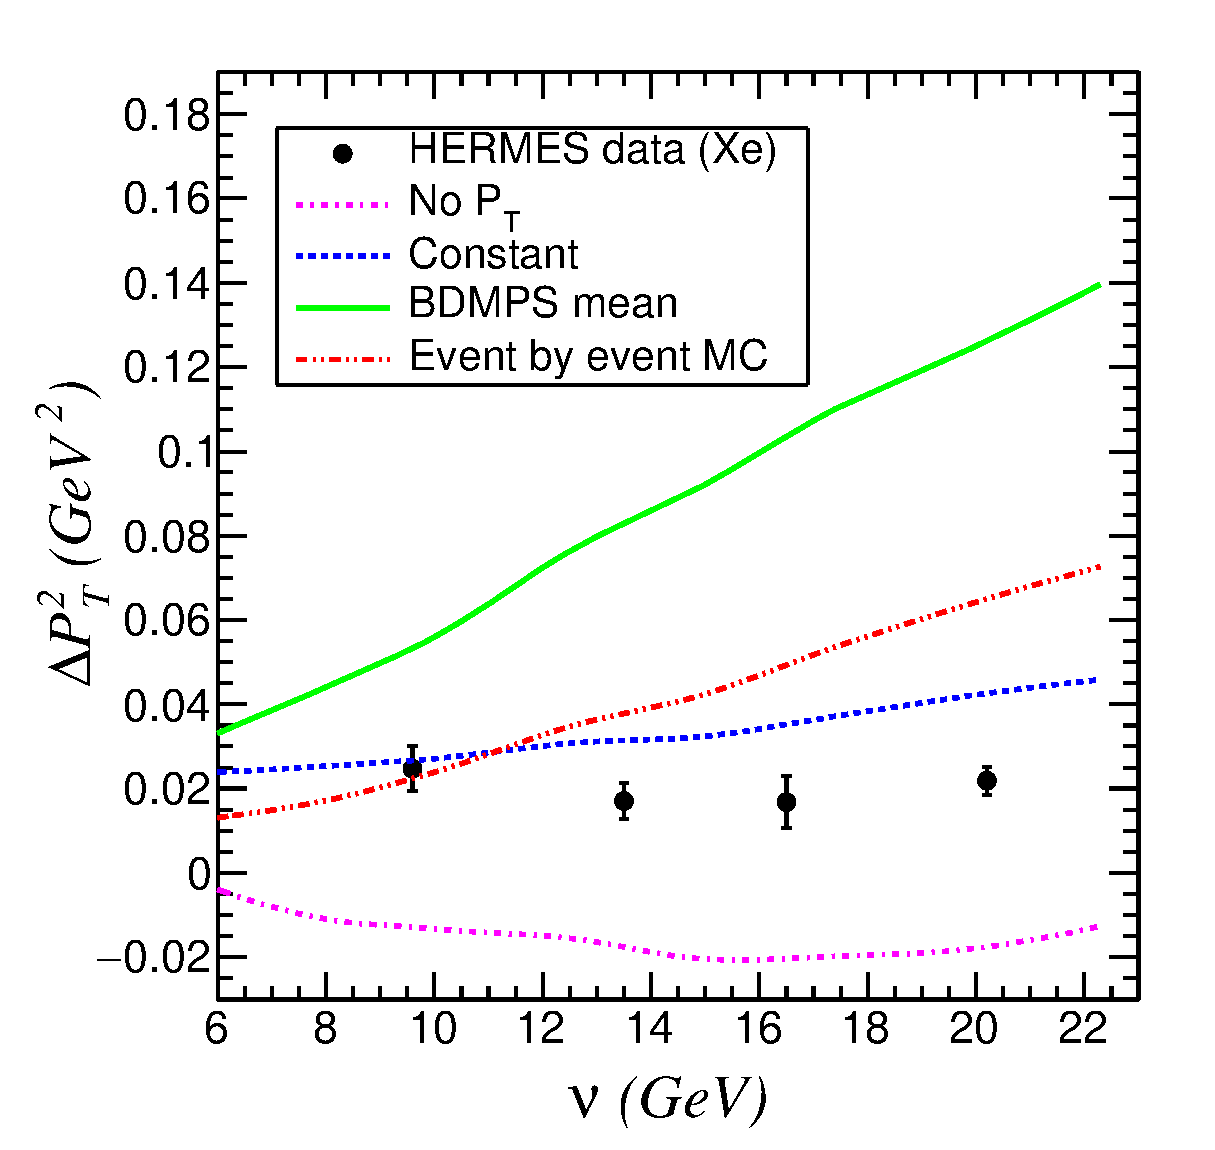
\includegraphics{fig/DPts_Nu_Comp.eps} }
\caption {Transverse momentum broadening of xenon as a function of $\nu$. 
HERMES data \cite{Airapetian:2009jy} (points) are compared with Monte-Carlo 
simulation (lines) for different transverse momentum broadening implementations 
(see section~\ref{sec:ptbroad}).}
\label{fig:PtC-PtNu}
\end{figure}

The result from HERMES \cite{Airapetian:2009jy}, shown in figure~%
\ref{fig:PtC-PtNu}, indicates that $\Delta P_T^2$ is constant with respect to 
$\nu$, we see here that this observation has important consequences on models. 
The BDMPS based simulation gives too much transverse momentum broadening and 
miss completely the data with an important dependence of $\Delta P_T^2$ to 
$\nu$. But the two other models gives values coherent with the measurement and 
reproduce the flat result from HERMES much better. In particular, the constant 
implementation of transverse momentum to all partons, directly based on 
$\qhat$, gives a result very close to the data. We also notice that the option 
without $p_T$ gives a slightly negative result, coherent with the negative 
Cronin effect observed previously.

\begin{figure}[tbp]
  \centering
\resizebox{0.45\textwidth}{!}{
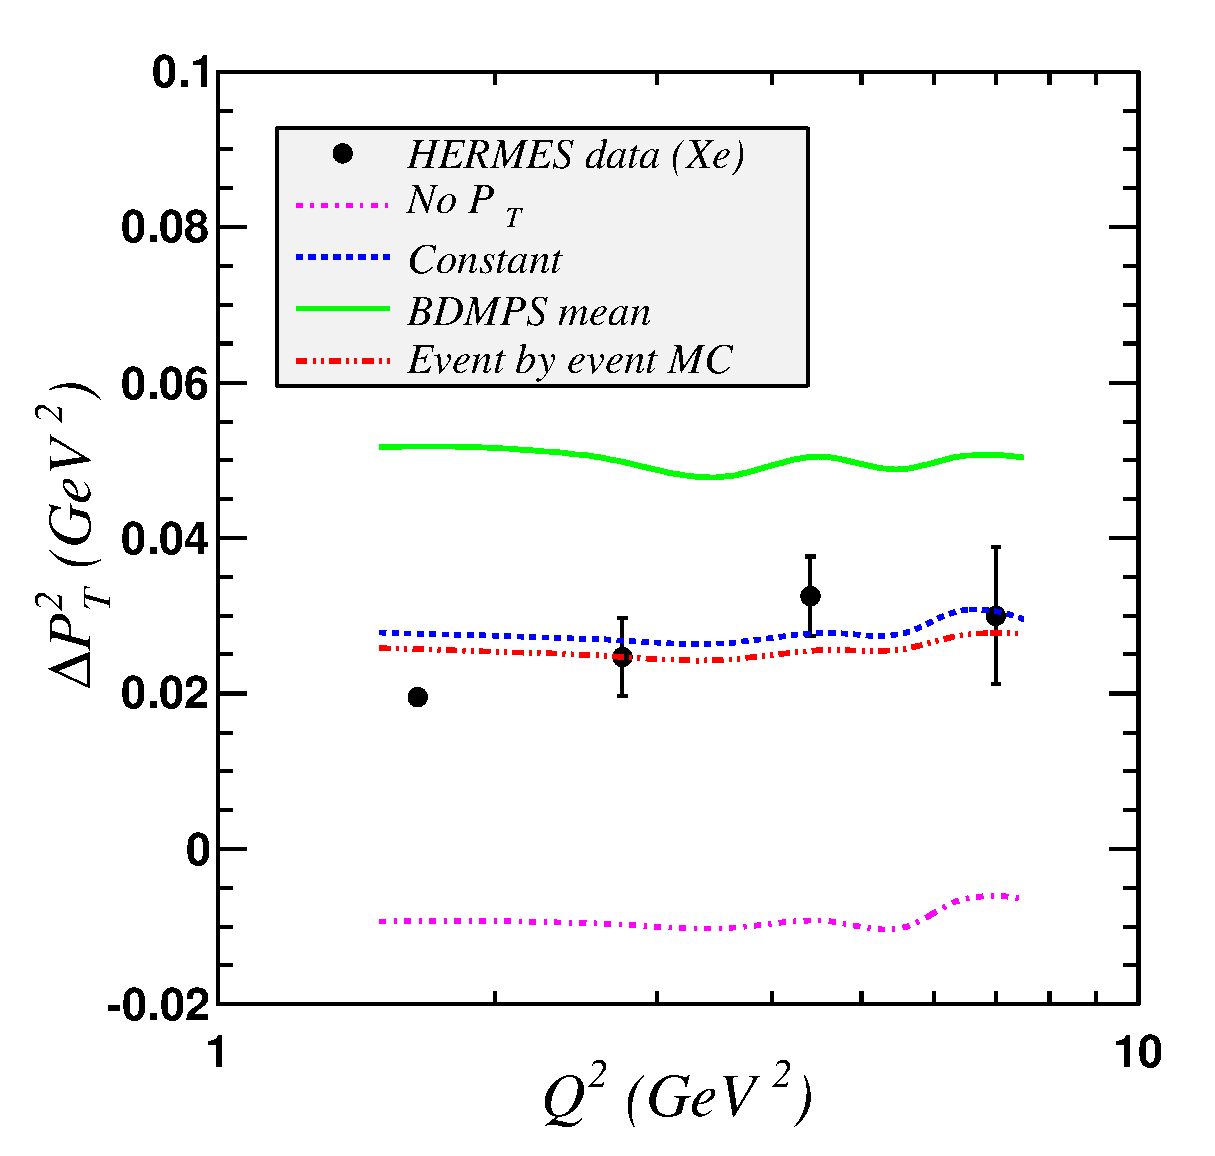
\includegraphics{fig/DPts_Q2_Comp.eps} }
\caption {Transverse momentum broadening of xenon as a function of $Q^2$. 
HERMES data \cite{Airapetian:2009jy} (points) are compared with Monte-Carlo 
simulation (lines) for different transverse momentum broadening implementations 
(see section~\ref{sec:ptbroad}).}
\label{fig:PtC-PtQ2}
\end{figure}

The results as function of $Q^2$, presented in figure~\ref{fig:PtC-PtQ2}, are 
flat for all models, which is coherent with data \cite{Airapetian:2009jy}. 
Again here the magnitude of $\Delta P_T^2$ is best reproduced by the constant 
and event by event MC models.

\begin{figure}[tbp]
  \centering
\resizebox{0.45\textwidth}{!}{
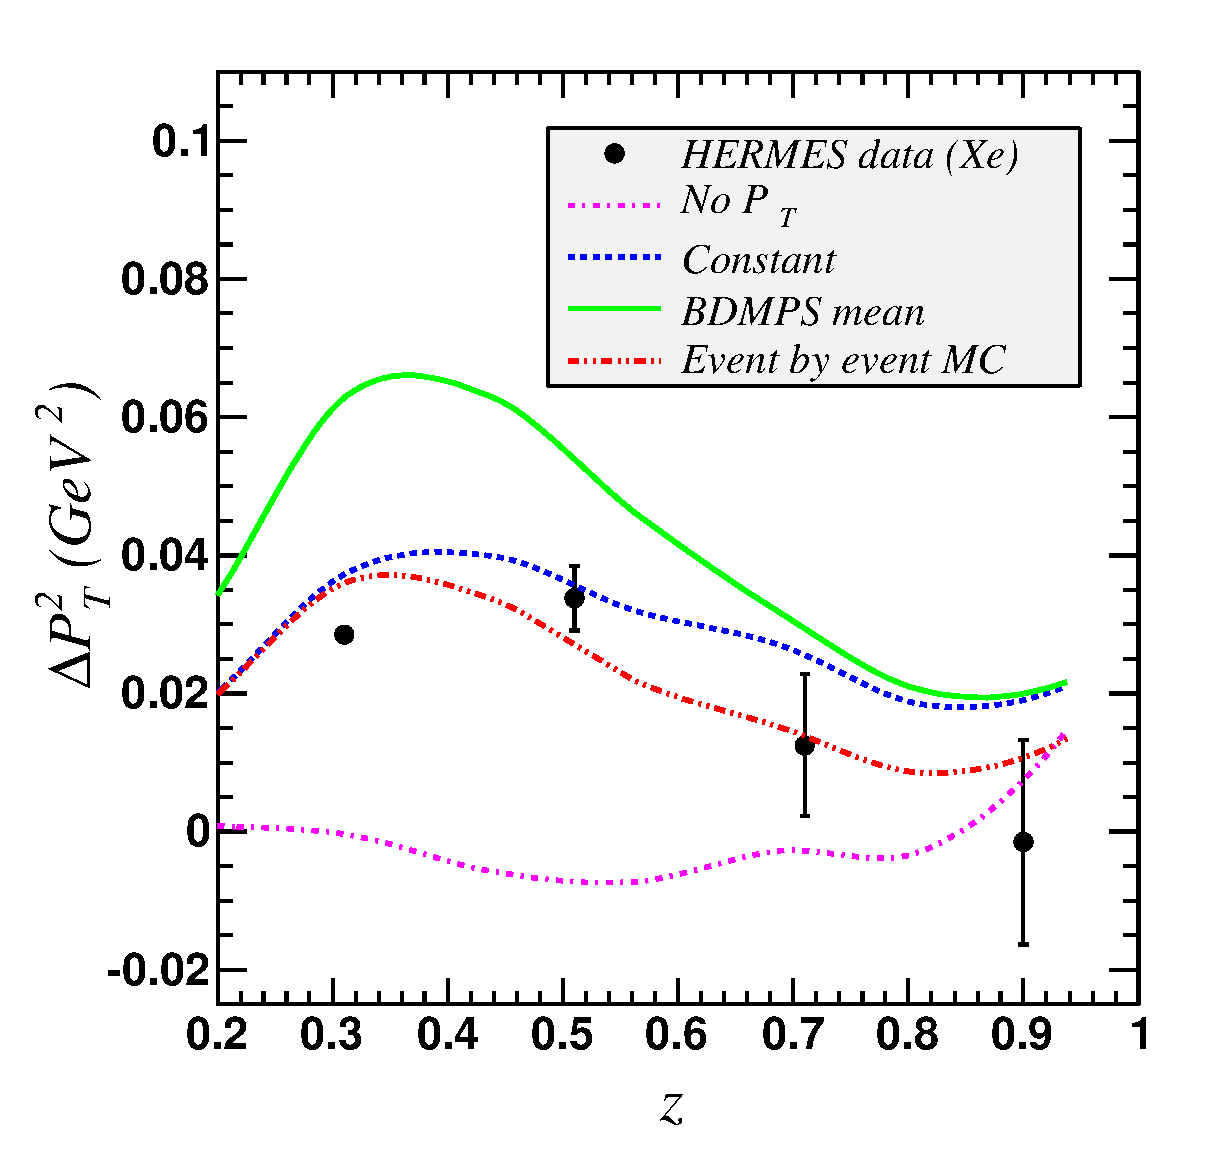
\includegraphics{fig/DPts_Z_Comp.eps} }
\caption {Transverse momentum broadening of xenon as a function of $z$. HERMES 
data \cite{Airapetian:2009jy} (points) are compared with Monte-Carlo simulation 
(lines) for different transverse momentum broadening implementations (see 
section~\ref{sec:ptbroad}).}
\label{fig:PtC-Ptz}
\end{figure}

HERMES results on $\Delta P_T^2$ as a function of $z$, in figure~%
\ref{fig:PtC-Ptz}, gives a puzzling result. Indeed, the position of the peak is 
expected to be at $z\gtrsim 0.7$ for pure energy loss models and in general all 
mixed models attributing $\Delta P_T^2$ effects to parton energy loss (see~%
\cite{Accardi:2009qv}, section 8.1.3 for full discussion). Our MC simulation 
does not appear to reproduce this feature of the models and peaks at much lower 
$z$, yet it offers a better match with the data. The best fit being the event 
by event MC implementation. This good result is one more indication that the 
correlation between the absorption effects and the transverse momentum 
broadening is important and correctly handled in this case. Indeed, the partons 
going through a long path in the nuclei are more affected by both transverse 
momentum broadening and quenching. Therefore, they might not lead to the 
production of hadrons in our detection window ($z>0.2$ at HERMES). For this 
reason we should not observe in the hadrons all the transverse momentum 
transferred to the partons. This explains the important discrepancy between our 
MC based method and a simple scaling of $\qhat$ by $z^2$ to obtain $\Delta 
P_T^2$.


\subsection{Atomic number dependence}

\begin{figure}[tbp]
  \centering
\resizebox{0.45\textwidth}{!}{
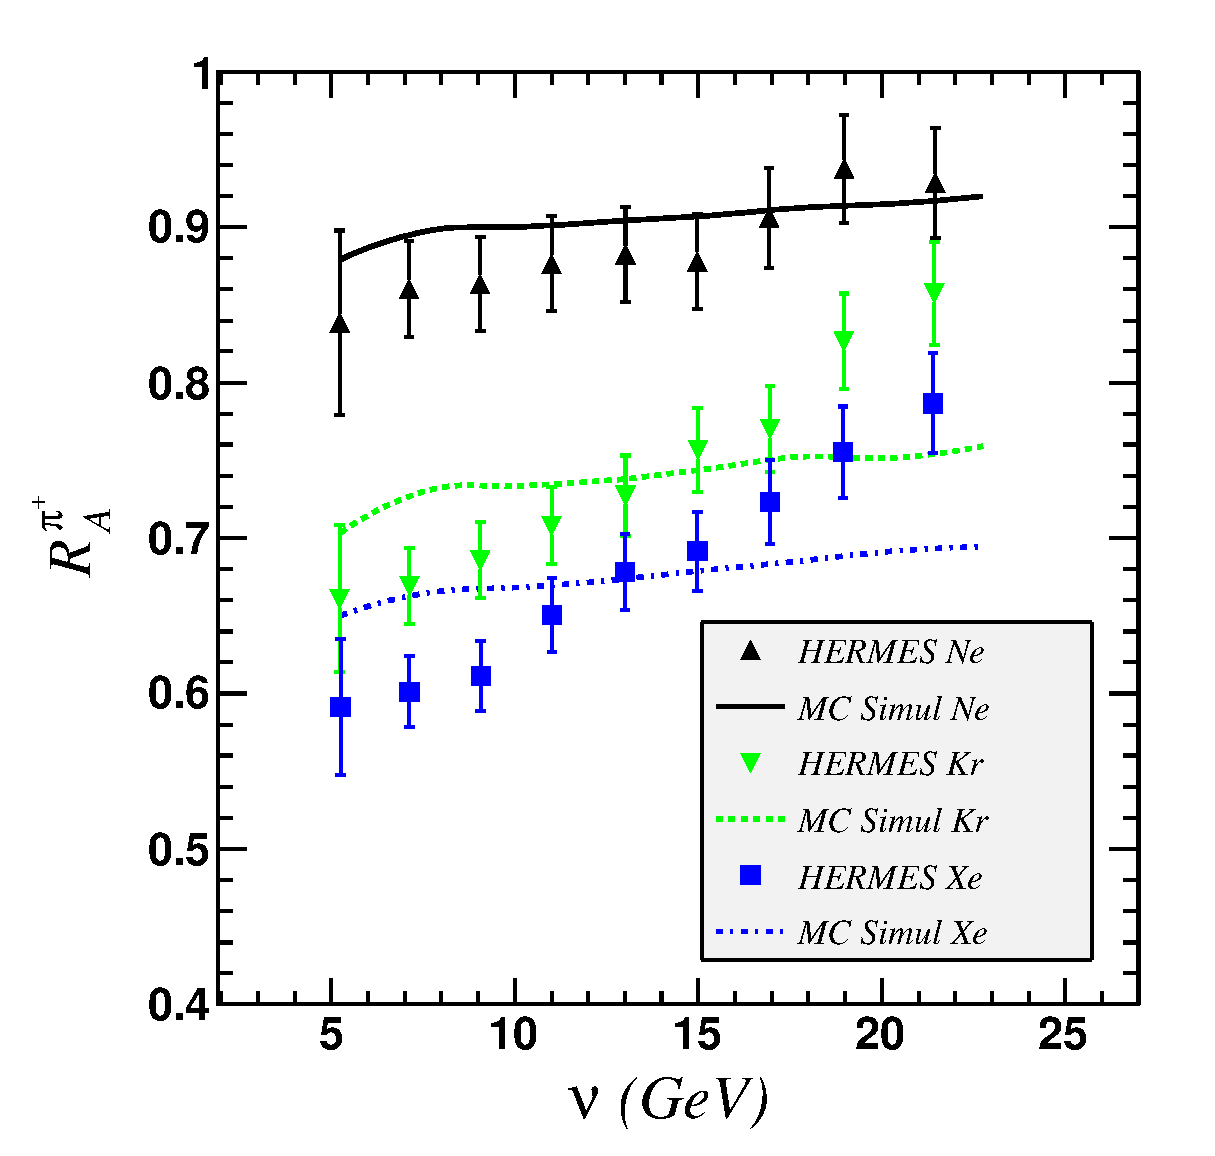
\includegraphics{fig/Ratio_Nu.eps} }
\caption {Multiplicity ratio as a function of $\nu$ for neon, krypton and 
xenon. HERMES data \cite{Airapetian:2011jp} (points) are compared with 
Monte-Carlo simulation (lines).}
\label{fig:RNu}
\end{figure}


\begin{figure}[tbp]
  \centering
\resizebox{0.45\textwidth}{!}{
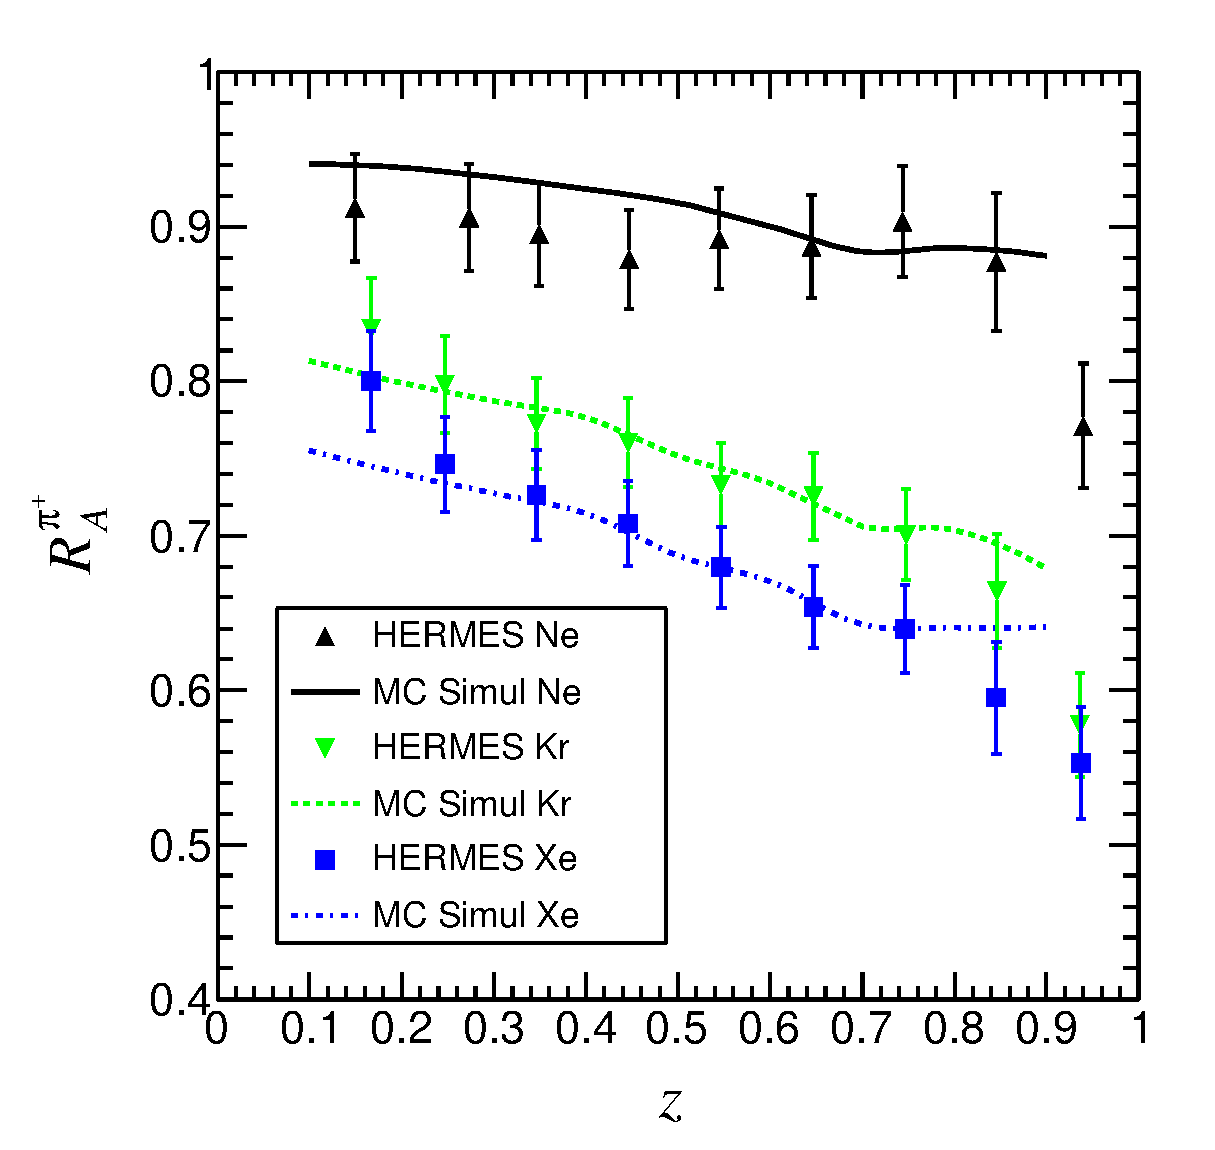
\includegraphics{fig/Ratio_Z.eps} }
\caption {Multiplicity ratio as a function of $z$ for neon, krypton and xenon. 
HERMES data \cite{Airapetian:2011jp} (points) are compared with Monte-Carlo 
simulation (lines).}
\label{fig:Rz}
\end{figure}

We present in figures~\ref{fig:RNu} and~\ref{fig:Rz} the results of our 
simulation using the event by event MC method to generate the transverse 
momentum. The simulation is compared to data for neon, krypton and xenon nuclei 
in order to illustrate the $A$ dependence of the multiplicity ratio. The result 
appears to be consistent with the data and we also confirm that the dependence 
to $z$ is properly described by our model. This is confirming the compatibility 
of the pure parton energy loss model with experimental data. However, the 
slopes observed as function of $\nu$ in figure~\ref{fig:RNu} indicate a 
significant mismatch between the model and data from all targets. This 
difference seem to indicate a problem with the quenching calculation or the 
parton generator, that lead to an incorrect trend as function of the virtual 
photon energy energy.

\begin{figure}[tbp]
  \centering
\resizebox{0.45\textwidth}{!}{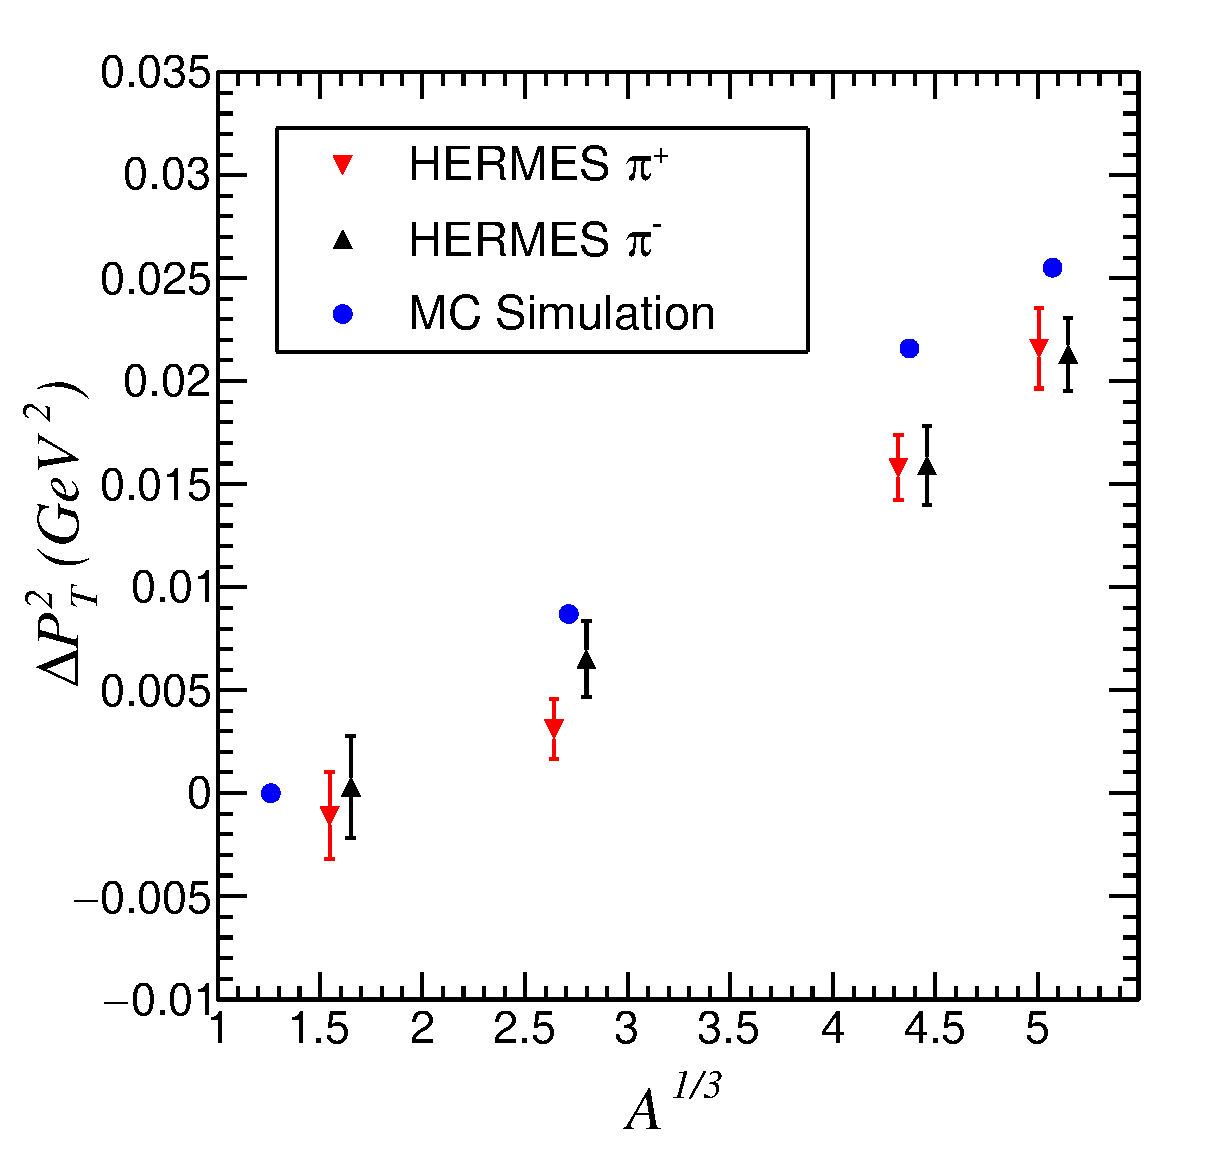
\includegraphics{fig/DPts_A_Comp.eps}}
\caption {Transverse momentum broadening as a function of $A^{1/3}$. HERMES 
data \cite{Airapetian:2009jy} (triangles) are compared with Monte-Carlo 
simulation (circles).}
\label{fig:PtA}
\end{figure}

Finally, in figure~\ref{fig:PtA}, we show our results obtained with the event 
by event MC generated transverse momentum, which indicates a good agreement 
between the model and the data~\cite{Airapetian:2009jy}. This was not expected 
from previous studies indicating an important gap between a small $\qhat$ 
extracted from $\Delta P_T^2$ and a large one necessary to describe the 
attenuation observed. However, we shown that the translation of the partonic 
$\qhat$ into the hadronic $\Delta P_T^2$ is not straight forward and needs 
precise study. Therefore, the correlation between attenuation and transverse 
momentum obtained in our MC, which describe the data properly, is an important 
confirmation of our extraction of $\qhat = 0.36\ \text{GeV}^2/ \text{fm}$.

{\bf [AA] Should we present the result as function of Lc somewhere in the section? We might keep that just for a proceeding. Another idea is to present ``predictions'' for JLab 6 energy, to see eventually the deviation fro $A^{1/3}$ inthe experimental data when published.}


\section{Conclusion}

We shown that Fermi motion has negligible effects on multiplicity ratios and 
small effects on $\Delta P_T^2$, which can be accounted for easily at HERMES 
energy. However, more significant effects are to be expected at lower energy 
experiments such as the one from the CLAS collaboration~%
\cite{Brooks:2009xg,DupreQNP}. We also show that this problem can be suppressed 
by using carbon nuclei instead of deuterium as reference nuclei in the 
hadronization observables. 

The description of the multiplicity ratios from HERMES~\cite{Airapetian:2007vu} 
with our MC simulation lead to the setting of our only parameter $\qhat = 0.36\ 
\text{GeV}^2/\text{fm}$. At this value, the calculation describes very well the 
$z$ dependence, but does not seem to reproduce properly the $\nu$ dependence. 
This might be due to a problem of the quenching weight calculation, yet it is 
difficult to rule out other possible sources. However, the good description of 
$\Delta P_T^2$ with the same setting is particularly striking. Indeed, the 
Monte-Carlo event by event generator gives access to complicated and intricate 
effects between fragmentation and nuclear effects. We analyzed this in more 
details with the comparison between the different models of parton transverse 
momentum broadening and showed the direct but complicated link with the 
observable $\Delta P_T^2$. In particular, we observe that the link between the 
transverse momentum of the parton and the one observed on hadrons is strongly 
affected by the hadron attenuation. This difficulty is making the MC procedure 
the most reliable to describe this observable. 

We also observed, as many previous work~\cite{Accardi:2009qv}, that the 
description of the multiplicity ratio as function of $z$ is relatively easy. 
The trend being dominated by the fragmentation function behavior not the 
nuclear attenuation model details. However, the reduction of the attenuation 
with $\nu$ seem to be much more sensitive to the detail of the model. Indeed, 
our model using Salgado and Wiedemann calculation fail with this data. 
Therefore, it appears that the cold nuclear matter can provide a good test of 
parton energy loss calculations using existing data. We finally want to point 
out that such a test is much more stringent in nuclear SIDIS than in HIC 
because of the control over the kinematic of the moving parton and over the 
size of the static medium.

\section*{Acknowledgments}

We gratefully acknowledge useful and informative discussions with K.~Hafidi and W.~Horowitz and A.~Majumder. We also thank C.A.~Salgado for providing us with ASW quenching weights for $R \geq 1$, and P.~Skands for help with parton handling in Pythia.
This work was partly supported by the DOE contract No.~DE-AC05-06OR23177,
under which Jefferson Science Associates, LLC operates Jefferson Lab, and by the DOE contract No. DE-SC008791.


\bibliographystyle{epj}
\bibliography{hadro}


\end{document}

% end of file template.tex
%% For one-column wide figures use
%\begin{figure}
%  \centering
%\resizebox{0.45\textwidth}{!}{%
%  
\includegraphics{leer.eps}
%}
%\caption{Please write your figure caption here}
%\label{fig:1}       % Give a unique label
%\end{figure}
%%
%% For two-column wide figures use
%\begin{figure*}
%\vspace*{5cm}       % Give the correct figure height in cm
%\caption{Please write your figure caption here}
%\label{fig:2}       % Give a unique label
%\end{figure*}
%%
%% For tables use
%\begin{table}
%\caption{Please write your table caption here}
%\label{tab:1}       % Give a unique label
%% For LaTeX tables use
%\begin{tabular}{lll}
%\hline\noalign{\smallskip}
%first & second & third  \\
%\noalign{\smallskip}\hline\noalign{\smallskip}
%number & number & number \\
%number & number & number \\
%\noalign{\smallskip}\hline
%\end{tabular}
%% Or use
%\vspace*{5cm}  % with the correct table height
%\end{table}
%%
